\chapter{Sistema de visión artificial}
\label{chap:Sistema de visión artificial}
\Abstract{En este capítulo se van a desarrollar los tres componentes que constituyen el sistema de visión artificial. Una primera red para identificar las piezas, una red intermedia para distinguir regiones de interés y una última capa para determinar los puntos de agarre.}

El fin de este proyecto es la generación de un nuevo sistema de visión artificial para el reconocimiento de piezas de uso industrial. Este sistema se implantará dentro de una cadena de suministro del Grupo Antolín\textsuperscript{\textregistered} que a su vez alimentará a una linea de montaje y ensamblaje. El sistema deberá de poder identificar múltiples piezas y determinar el punto de agarre óptimo de cada pieza. Este se ve definido por sus coordenadas así como el vector normal a la superficie. De esta forma un brazo robótico con un sistema de agarre por aspiración, ventosa o \textit{soft-robotics} (varía en función de la pieza a coger) podrá recolectarlas.

La multitud de herramientas de agarre así como de la necesidad de un sistema de determinación de puntos de agarre se debe a la gran variedad de piezas existentes con formas y tamaños de gran variedad (1-30 cm). Esto ha obligado el desarrollo de un sistema modular capaz de adaptarse dependiendo del tamaño de la pieza. Se ha definido un primer proceso común para todas las piezas basado en YOLOv5 que permite la identificación de las piezas. Para las piezas pequeñas se empleará el punto medio de la pieza identificada como punto de agarre. Sin embargo, esta lógica no se puede emplear para las piezas grandes debido a su complejidad y a las superficies irregulares. Por ello, se ha definido un proceso adicional que parte de a salida de YOLO y es capaz de determinar el punto de agarre óptimo. El proceso esta a su vez constituido por dos etapas.

\begin{itemize}
\item YOLO: consiste en una red convolucional del tipo YOLOv5 de gran tamaño. Se encarga de identificar y detectar las piezas presentes en el entorno de trabajo. Para recolectar las piezas pequeñas se empleará el punto medio de la pieza y un vector perpendicular a la superficie de trabajo. Sin embargo, para las piezas grandes se requiere de un proceso más avanzado basado en Tiny YOLO y un regresor.
\item Tiny YOLO: como su nombre indica, se trata de una red convolucional del tipo YOLO pero de menor tamaño capaz de determinar para una pieza sus regiones con posibles puntos de agarre.
\item Regresor: se trata de una red neuronal convolucional del tipo regresor capaz de determinar para las regiones de interés de cada pieza el punto de agarre. Este está definido por las coordenadas así como el vector normal a dicho punto.
\end{itemize}

El uso de una capa intermedia (Tiny YOLO) se debe a la naturaleza de un regresor. Este tipo de red es capaz de estimar para una pieza dad los diferentes puntos de agarre. Pero no dispone ningún mecanismo que nos permita calcular la probabilidad de que ese punto haya sido determinado correctamente. Una forma clara de visualizar este concepto es suponer un escenario muy común en la práctica. Supongamos que una pieza está dada la vuelta de forma que el punto de agarre se encuentre apuntando al suela. En la práctica esta pieza no puede ser recolectada por el brazo robótico ya que no tiene acceso al punto de agarre. Por lo que la salida del sistema debería de ser nula. Sin embargo, debido a la naturaleza de los regresores, este intentará determinar el punto de agarre aunque no pueda verlo y este no sea accesible. Es debido a esto que se debe de emplear una capa intermedia que determine si el punto que se quiere agarrar es accesible por el robot o no.

\begin{figure}[ht]
	\centering
	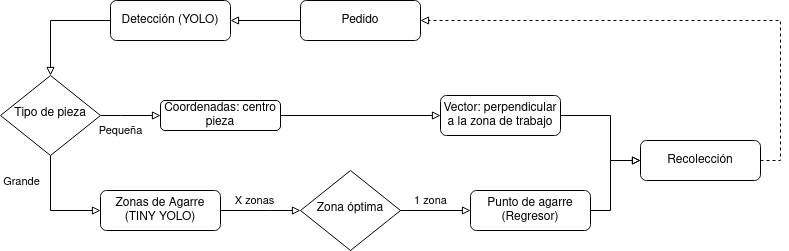
\includegraphics[width=1\textwidth]{Sistema de vision artificial/Diagrama_vision.png}
	\caption{Esquema de la arquitectura del sistema}
	\label{chap:Sistema de visión artificial fig:Arquitectura generador}
\end{figure}

\vspace{5pt}
\begin{table}[ht]
	\centering
	\begin{tabular}{|c|c|}
	\hline 
	SO & Ubuntu 18.04 \\
	\hline
	Kernel &  5.15.0-40-generic \\
	\hline 
	Procesador & Intel Core i5-8250U @ 3.40GHz \\ 
	\hline 
	Nucleos/Hilos & 4/8 \\
	\hline
	Ram & 16 GB 2666 MHz\\ 
	\hline 
	GPU & Intel UHD 620 \\ 
	\hline 
	\end{tabular} 
	\caption{Ordenador empleado para el entrenamiento}
	\label{chap:Sistema de visión artificial tab:Ordenador}
\end{table}
\vspace{5pt}


\section{YOLO}
\label{chap:Sistema de visión artificial sec:YOLO}
En 2015 se produjo una revolución que cambió la forma de trabajar con las redes neuronales y nuestro entendimiento de estas. En 2015 cuatro investigadores de la universidad de Washington desarrollaron un nuevo tipo de red neuronal bautizada como YOLO (You Only Look Once) \citep{YOLO}. Esta nueva red se caracteriza porque tal y como su nombre indica, la imagen solo se analiza una vez. Esto puede parecer similar a redes como Faster R-CNN pero difiere bastante. En Faster R-CNN la imagen es inicialmente procesada por las capas de convolución para a continuación determinar regiones de interés con la ayuda de una red tipo RPN. Finalmente, se analiza cada una de las posibles regiones de interés por separado. Esto implica qué aunque inicialmente la imagen pase completamente por las capas de convolución, después se analiza por secciones por lo tanto es necesario analizar la misma imagen varias veces.

Sin embargo, esto no sucede en YOLO por la forma interna en la que trabaja. YOLO no fue diseñada con la idea de reaprovechar un clasificador ya existente para detectar objetos, se construyo desde cero y con el único objetivo de detectar objetos. Es decir, para detectar objetos no recurre a la técnica de correr un clasificador por diferentes regiones de la imagen y así detectar un objeto. YOLO emplea un método completamente diferente, este comienza por la división de la imagen en secciones, en el artículo original, se divide la imagen en una 7x7 secciones, aunque el número de secciones se pueden modificar. Para cada una de las secciones una capa convolucional predice un número de posibles \textit{bounding boxes} (área de la imagen que puede contener un objeto) así como la posible clase de cada \textit{bounding box} y su probabilidad de ser ese objeto. Por último, se analizan en conjunto todos los \textit{bounding boxes} definidos así como su clase y su probabilidad y se determina cuáles son los objetos en la imagen y donde están.

\begin{figure}[ht]
	\centering
	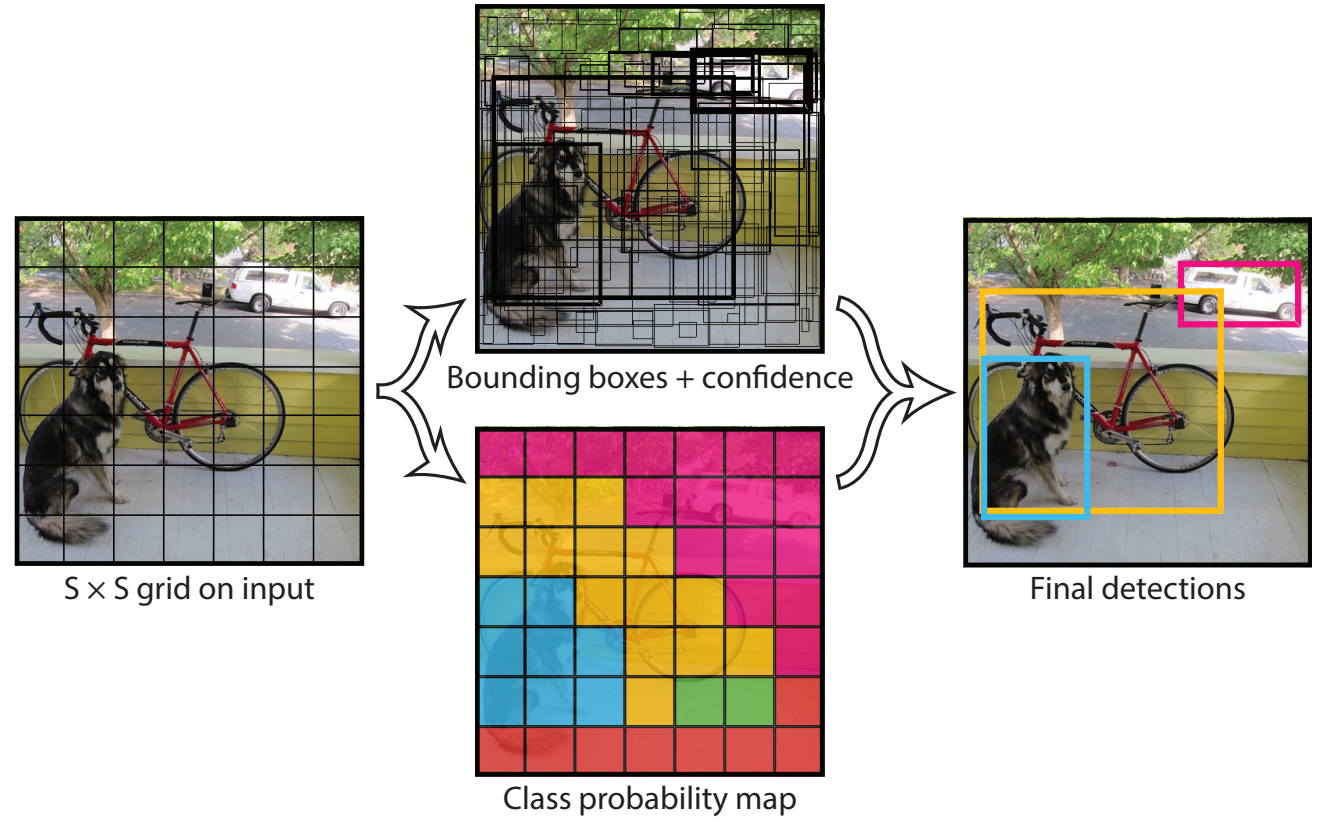
\includegraphics[width=0.7\textwidth]{Sistema de vision artificial/YOLO/esquema_funcionamiento.png}
	\caption[Esquema del funcionamiento de YOLO]{Esquema del funcionamiento de YOLO (Fuente: publicación original de YOLO \citep{YOLO})}
	\label{chap:Sistema de visión artificial fig:Funcionamiento YOLO}
\end{figure}

Este método presenta numerosas ventajas frente a R-CNN y Faster R-CNN, en primer lugar, destaca por su rapidez. La primera red diseñada por los desarrolladores de YOLO cuenta con con 24 capas de convolución y era capaz de correr a 45 imágenes por segundo (gracias a avances en computación actualmente es capaz de correr con una mayor tasa de refresco). Esta red también se caracteriza por tener una estructura más propia de las Fully Convolutional Neuronal Network (FCNN), es decir, se caracteriza por ser mayoritariamente convolucional. Otra de sus grandes ventajas, es que al mirar a la imagen entera, es capaz de ver la diferentes conexiones entre \textit{bounding boxes} y determinar de forma rápida y precisa la posición del objeto. Esto no ocurre en métodos como la ventana flotante. A continuación, se muestra de forma breve y gráfica el funcionamiento de YOLO en la \autoref{chap:Sistema de visión artificial fig:Funcionamiento YOLO}

\subsection{Estructura}
\label{chap:Sistema de visión artificial subsec:YOLO Estructura}
Debido al gran interés y las capacidades de YOLO, este ha sido desarrollado bastante en los últimos años. En la actualidad se han publicado cinco versiones de YOLO que mejoran su rendimiento y le dotan de más capacidades. Estas nuevas versiones han traído consigo cambios en la estructura de principal de YOLO para mejorar sus capacidades y rendimiento. A la vez se han desarrollado variantes de la red principal de diferentes tamaños con el fin de poder implantar estos sistemas en sistemas con capacidades computacionales menores. Para el desarrollo de este proyecto nos basaremos en la última versión disponible, la versión cinco que trae consigo un total de diez modelos de diferentes tamaños y resoluciones (ver \autoref{chap:Sistema de visión artificial tab:YOLO models}).

La primera red neuronal del sistema de visión artificial se basará en el modelo YOLOv5l que se caracteriza por mantener una buena relación entre potencia y capacidades. Este será el modelo capaz de distinguir e identificar todas las piezas y es por ello que requiere de una mayor capacidad. Se puede observar la estructura interna de la red en \autoref{apex:Estructura YOLOv5}.

\begin{table}[ht]
	\centering
	\begin{tabular}{|c|c|c|c|c|c|c|c|}
	\hline 
	Model
	& \begin{tabular}{@{}c@{}}Size \\ {\footnotesize (pixels)}\end{tabular}
	& \begin{tabular}{@{}c@{}}$mAP^{val}$ \\ {\footnotesize 0.5:0.95}\end{tabular}
	& \begin{tabular}{@{}c@{}}$mAP^{val}$ \\ {\footnotesize 0.5}\end{tabular}
	& \begin{tabular}{@{}c@{}c@{}}Speed \\ {\footnotesize V100 b1} \\ {\footnotesize (ms)}\end{tabular}
	& \begin{tabular}{@{}c@{}c@{}}Speed \\ {\footnotesize V100 b32} \\ {\footnotesize (ms)}\end{tabular}
	& \begin{tabular}{@{}c@{}}Params \\ {\footnotesize (M)}\end{tabular}
	& \begin{tabular}{@{}c@{}}FLOPs \\ {\footnotesize @640 (B)}\end{tabular}
	\\
	\hline 
	YOLOv5n & 640 & 28.0 & 45.7 & 6.3 & 0.6 & 1.9 & 4.5 \\ 
	\hline 
	YOLOv5s & 640 & 37.4 & 56.8 & 6.4 & 0.9 & 7.2 & 16.5 \\ 
	\hline 
	YOLOv5m & 640 & 45.4 & 64.1 & 8.2 & 1.7 & 21.2 & 49.0 \\ 
	\hline 
	YOLOv5l & 640 & 49.0 & 67.3 & 10.1 & 2.7 & 46.5 & 109.1 \\ 
	\hline 
	YOLOv5x & 640 & 50.7 & 68.9 & 12.1 & 4.8 & 86.7 & 205.7 \\ 
	\hline 
%	\hline 
	YOLOv5n6 & 1280 & 36.0 & 54.4 & 8.1 & 2.1 & 3.2 & 4.6 \\ 
	\hline 
	YOLOv5s6 & 1280 & 44.8 & 63.7 & 8.2 & 3.6 & 12.6 & 16.8 \\ 
	\hline 
	YOLOv5m6 & 1280 & 51.3 & 69.3 & 11.1 & 6.8 & 35.7 & 50.0 \\ 
	\hline 
	YOLOv5l6 & 1280 & 53.7 & 71.3 & 15.8 & 10.5 & 76.8 & 111.4 \\ 
	\hline 
	\begin{tabular}{@{}c@{}}YOLOv5x6 \\ + TTA\end{tabular}
	& \begin{tabular}{@{}c@{}}1280 \\ 1536\end{tabular}
	& \begin{tabular}{@{}c@{}}55.0 \\ 55.8\end{tabular}
	& \begin{tabular}{@{}c@{}}72.7 \\ 72.7\end{tabular}
	& \begin{tabular}{@{}c@{}}26.2 \\ -\end{tabular}
	& \begin{tabular}{@{}c@{}}19.4 \\ -\end{tabular}
	& \begin{tabular}{@{}c@{}}140.7 \\ -\end{tabular}
	& \begin{tabular}{@{}c@{}}209.8 \\ -\end{tabular}
	\\ 
	\hline 
	\end{tabular} 
	\caption{Modelos de YOLOv5}
	\label{chap:Sistema de visión artificial tab:YOLO models}
\end{table}

\subsection{Entrenamiento}
\label{chap:Sistema de visión artificial sec:YOLO Entrenamiento}
Una de las mejoras introducidas en YOLOv5 es la evolución de los hiperparámetros. Este nuevo sistema permite ejecutar numerosos entrenamientos bajo diferentes hiperparámetros con el objetivo de optimizar estos de forma automática. Para el desarrollo de esta red se ha empleado esta nueva función de forma que se ha podido reducir notablemente el tiempo de entrenamiento gracias a la reducción del proceso de aprendizaje en base a prueba y error.

Con el fin de obtener los mejores resultados posibles se ha optado por emplear el proceso evolutivo de YOLO. Se trata de un proceso iterativo en el que en base a una función objetivo se van seleccionando los hiperparámetros de entrenamiento con el fin de optimizar el entrenamiento. Estos nuevos hiperparámetros se obtienen por medio de un algoritmo genético, de forma que los mejores resultados de la anterior iteración se emplearán como base para la creación de nuevos hiperparámetros. La función objetivo empleada se caracteriza por ser una combinación de $mAP@0.5$ con una contribución del 10\% y $mAP@0.5:0.95$ con una contribución del 90\%.

\begin{lstlisting}[language=Python]
 def fitness(x): 
     # Model fitness as a weighted combination of metrics 
     w = [0.0, 0.0, 0.1, 0.9]  # weights for [P, R, mAP@0.5, mAP@0.5:0.95] 
     return (x[:, :4] * w).sum(1) 
\end{lstlisting}

Se recomienda realizar un mínimo de 300 iteraciones para poder obtener unos resultados óptimos. Sin embargo, debido a límites de tiempo y potencia se ha optado por reducir a 100 iteraciones y cada una con un total de 10 \textit{epochs}. En la \autoref{chap:Sistema de visión artificial tab:YOLO options} se muestran los hiperparámetros empleados durante todo el proceso.

\begin{table}[ht]
  \centering
    \begin{tabular}{|l|c|c|}
    \hline
    \multicolumn{3}{|c|}{Opciones de entrenamiento} \\
    \hline
    Parametro & Base & Evolución \\
    \hline
    Optimizador & \multicolumn{2}{|c|}{SGD momentum/Adam betal} \\
    \hline
    Initial learn rate & 0.01 & 0.00769 \\
    \hline
    Learn rate decay & 0.01 & 0.01464 \\
    \hline
    Momentum & 0.937 & 0.98 \\
    \hline
    Weight decay & 0.0005 & 0.00059 \\
    \hline
    Warmup epochs & 3.0 & 2.961 \\
    \hline
    Warmup momentun & 0.8 & 0.85061 \\
    \hline
    Box loss gain & 0.05 & 0.05199 \\
    \hline
    CLS loss gain & 0.5 & 0.4489 \\
    \hline
    IoU threshold & 0.2 & 0.2 \\
    \hline
    Anchor threshold & 4 & 4.6172 \\
    \hline
    Epochs & 100 & 100 \\
    \hline
    Batch Size & 16 & 16 \\
    \hline
    \end{tabular}
  \caption{Opciones de entrenamiento de YOLO}
  \label{chap:Sistema de visión artificial tab:YOLO options}
\end{table}

\subsection{Resultados}
\label{chap:Sistema de visión artificial sec:YOLO Resultados}
Con la ayuda de YOLO se ha podido realizar un último análisis del \textit{dataset} empleado con el fin de determinar las instancias, la ubicación y forma de los diferentes objetos presentes. Y determinar si existe alguna correlación entre estos. Analizando los resultados lo primero que se puede observar es la notable diferencia de instancias de piezas G1 y G3 respecto al resto de piezas pequeñas. El motivo principal de semejante diferencia es falta de tiempo y de potencia computacional para renderizar un mayor número de imágenes. Las pruebas iniciales del proyecto se realizaron con dichas piezas y es por ello que se dispone de un mayor número de instancias.

Analizando la posición de las piezas se observa que se cubre la totalidad del área de trabajo pero se observa un claro patrón cuadrático. Esto es debido a que los escenarios empleados presentan forma de cajas de tres tamaños, lo cual queda reflejado en la distribución de las piezas. Se observa también formas cuadradas dispersas por el interior de las cajas, estas son una adición al escenario con el fin de evitar que las piezas queden paralelas a la superficie de trabajo y aumentar así la riqueza del \textit{dataset}.

Si se analiza la forma de todas las instancias se comprueba que un elevado grado de dispersión pero siguiendo una ligera distribución lineal de forma que existe correlación entre el ancho y el alto de las instancias. Esto se debe a que todas las piezas empleadas presentan una forma rectangular con lados semejantes. Por último, se puede observa el tamaño de las instancias dividido en alto y ancho. Se puede observar en ambos histogramas la presencia de dos categorías de piezas, piezas grandes y piezas pequeñas. Las piezas pequeñas se muestran al inicio de ambos histogramas y presentan todas un tamaño muy similar. Por otro lado, las piezas grandes se encuentran distribuidas por el resto del histograma y presentan una mayor varianza.

\begin{figure}[ht]
  \subfloat{
	\begin{minipage}[c][1\width]{0.49\textwidth}
	   \centering
	   \includegraphics[width=1\textwidth]{Sistema de vision artificial/YOLO/base_YOLO/labels.jpg}
	\end{minipage}}
  \hfill	
  \subfloat{
	\begin{minipage}[c][1\width]{0.49\textwidth}
	   \centering
	   \includegraphics[width=1\textwidth]{Sistema de vision artificial/YOLO/base_YOLO/labels_correlogram.jpg}
	\end{minipage}}
\caption{Evaluación de instancias, forma y ubicación del \textit{dataset} empleado en YOLO}
\label{chap:Sistema de visión artificial fig:YOLO labels}
\end{figure}

Como se ha mencionado en la sección de entrenamiento, se ha empleado un algoritmo genético para la estimación de los hiperparámetros con el fin de mejorar los resultados de la red. Es por ello que en los resultados se comparará dos redes. Ambas han sido entrenadas el mismo número de \textit{epochs} pero con diferentes hiperparámetros. Se compararán los hiperparámetros definidos por defecto por los desarrolladores de YOLO y los definidos por el algoritmo evolutivo.

Los resultados del proceso evolutivo se dividen en dos secciones, en primer lugar se muestra en la \autoref{chap:Sistema de visión artificial fig:Evolución YOLO} el proceso de evolución de los hiperparámetros y como estos han ido cambiando entre las diferentes evoluciones. Y en segundo lugar, se muestra en la \autoref{chap:Sistema de visión artificial fig:Resultados evolución YOLO} una comparativa de los resultados de cada red entrenada durante el proceso evolutivo. Analizando estas dos gráficas se puede llegar a la falsa conclusión de que el sistema no ha sido capaz de optimizar los hiperparámetros debido a la aparente aleatoriedad de la distribución de los datos. Sin embargo, al comparar ambos modelos se observa grandes mejoras respecto al caso base tanto en entrenamiento como en validación. Es probable que la aparente aleatoriedad de los resultados se deba a una falta de \textit{epochs}. Con un número tan reducido es difícil hacer asunciones sobre los hiperparámetros. Si se desea obtener los resultados óptimos también se debe de considerar un aumento del número de iteraciones.

Una vez completado el proceso evolutivo se han entrenado las dos versiones de YOLO con diferentes hiperparámetros. En ambos casos se observa como la red neuronal es capaz de generalizar y extraer la información y características de las piezas. Pero también se observa la falta de entrenamiento ya que las métricas siguen mejorando cuando se detuvo el entrenamiento. Pero a pesar de ello se puede observar el gran rendimiento y capacidades de YOLO. También se observa una clara mejora al emplear los hiperparámetros obtenidos por el algoritmo evolutivo tanto en entrenamiento como en validación. Por último, una vez realizado el entrenamiento se ha analizado una nueva sección del \textit{dataset} que no ha sido empleada para entrenamiento ni para validación durante el entrenamiento. Con este nuevo \textit{dataset} se han obtenido unos resultados prometedores (ver \autoref{chap:Sistema de visión artificial fig:YOLO Val Matrix}) caracterizados por una tasa de fallos reducida y una precisión elevada para niveles de confianza del 50\%. Los resultados son prometedores pero esto no implica que sean perfectos. La red presenta una clara ligera tendencia a dar falsos positivos a la hora de detectar algunas de las piezas. Esto se debe a varios factores:

\begin{itemize}
\item Texturas: al emplear una librería de texturas no se tiene un control total sobre estas. Algunas de las texturas empleadas son de colores oscuros lo que dificulta en gran medida la detección de las piezas negras. Las piezas grandes no se ven tan afectadas por la presencia de mayor relieve.
\item Tamaño: Las piezas pequeñas se encuentran a una distancia elevada de la cámara y en ocasiones el área de la pieza se puede medir en decenas de píxeles.
\end{itemize}

Se recomiendo replantear la configuración del generador de imágenes para las piezas pequeñas. Como primera medida se debe de reducir la distancia a las piezas para obtener mayor detalle de las piezas. Si es posible se recomiendo no modificar las texturas para evitar sesgar el \textit{dataset.}

Por último, se ha obtenido la precisión y el \textit{recall} de validación (ver \autoref{chap:Sistema de visión artificial fig:YOLO Val PR}). Con la precisión se observa como con un nivel de confianza del 40\% se pueden obtener resultados con una precisión elevada. Y con \textit{recall} se observa como ha medida que aumentamos el nivel de confianza requerido aumenta el numero de falsos negativos (piezas no detectadas). En la curva F1 se enfrentan ambas métricas permitiendo ver de forma visual como afecta el nivel de confianza a la identificación de piezas. Se observa como el modelo final debe de trabajar con un nivel de confianza entre el 40\% y 80\% para obtener resultados óptimos.

\begin{figure}[H]
	\centering
	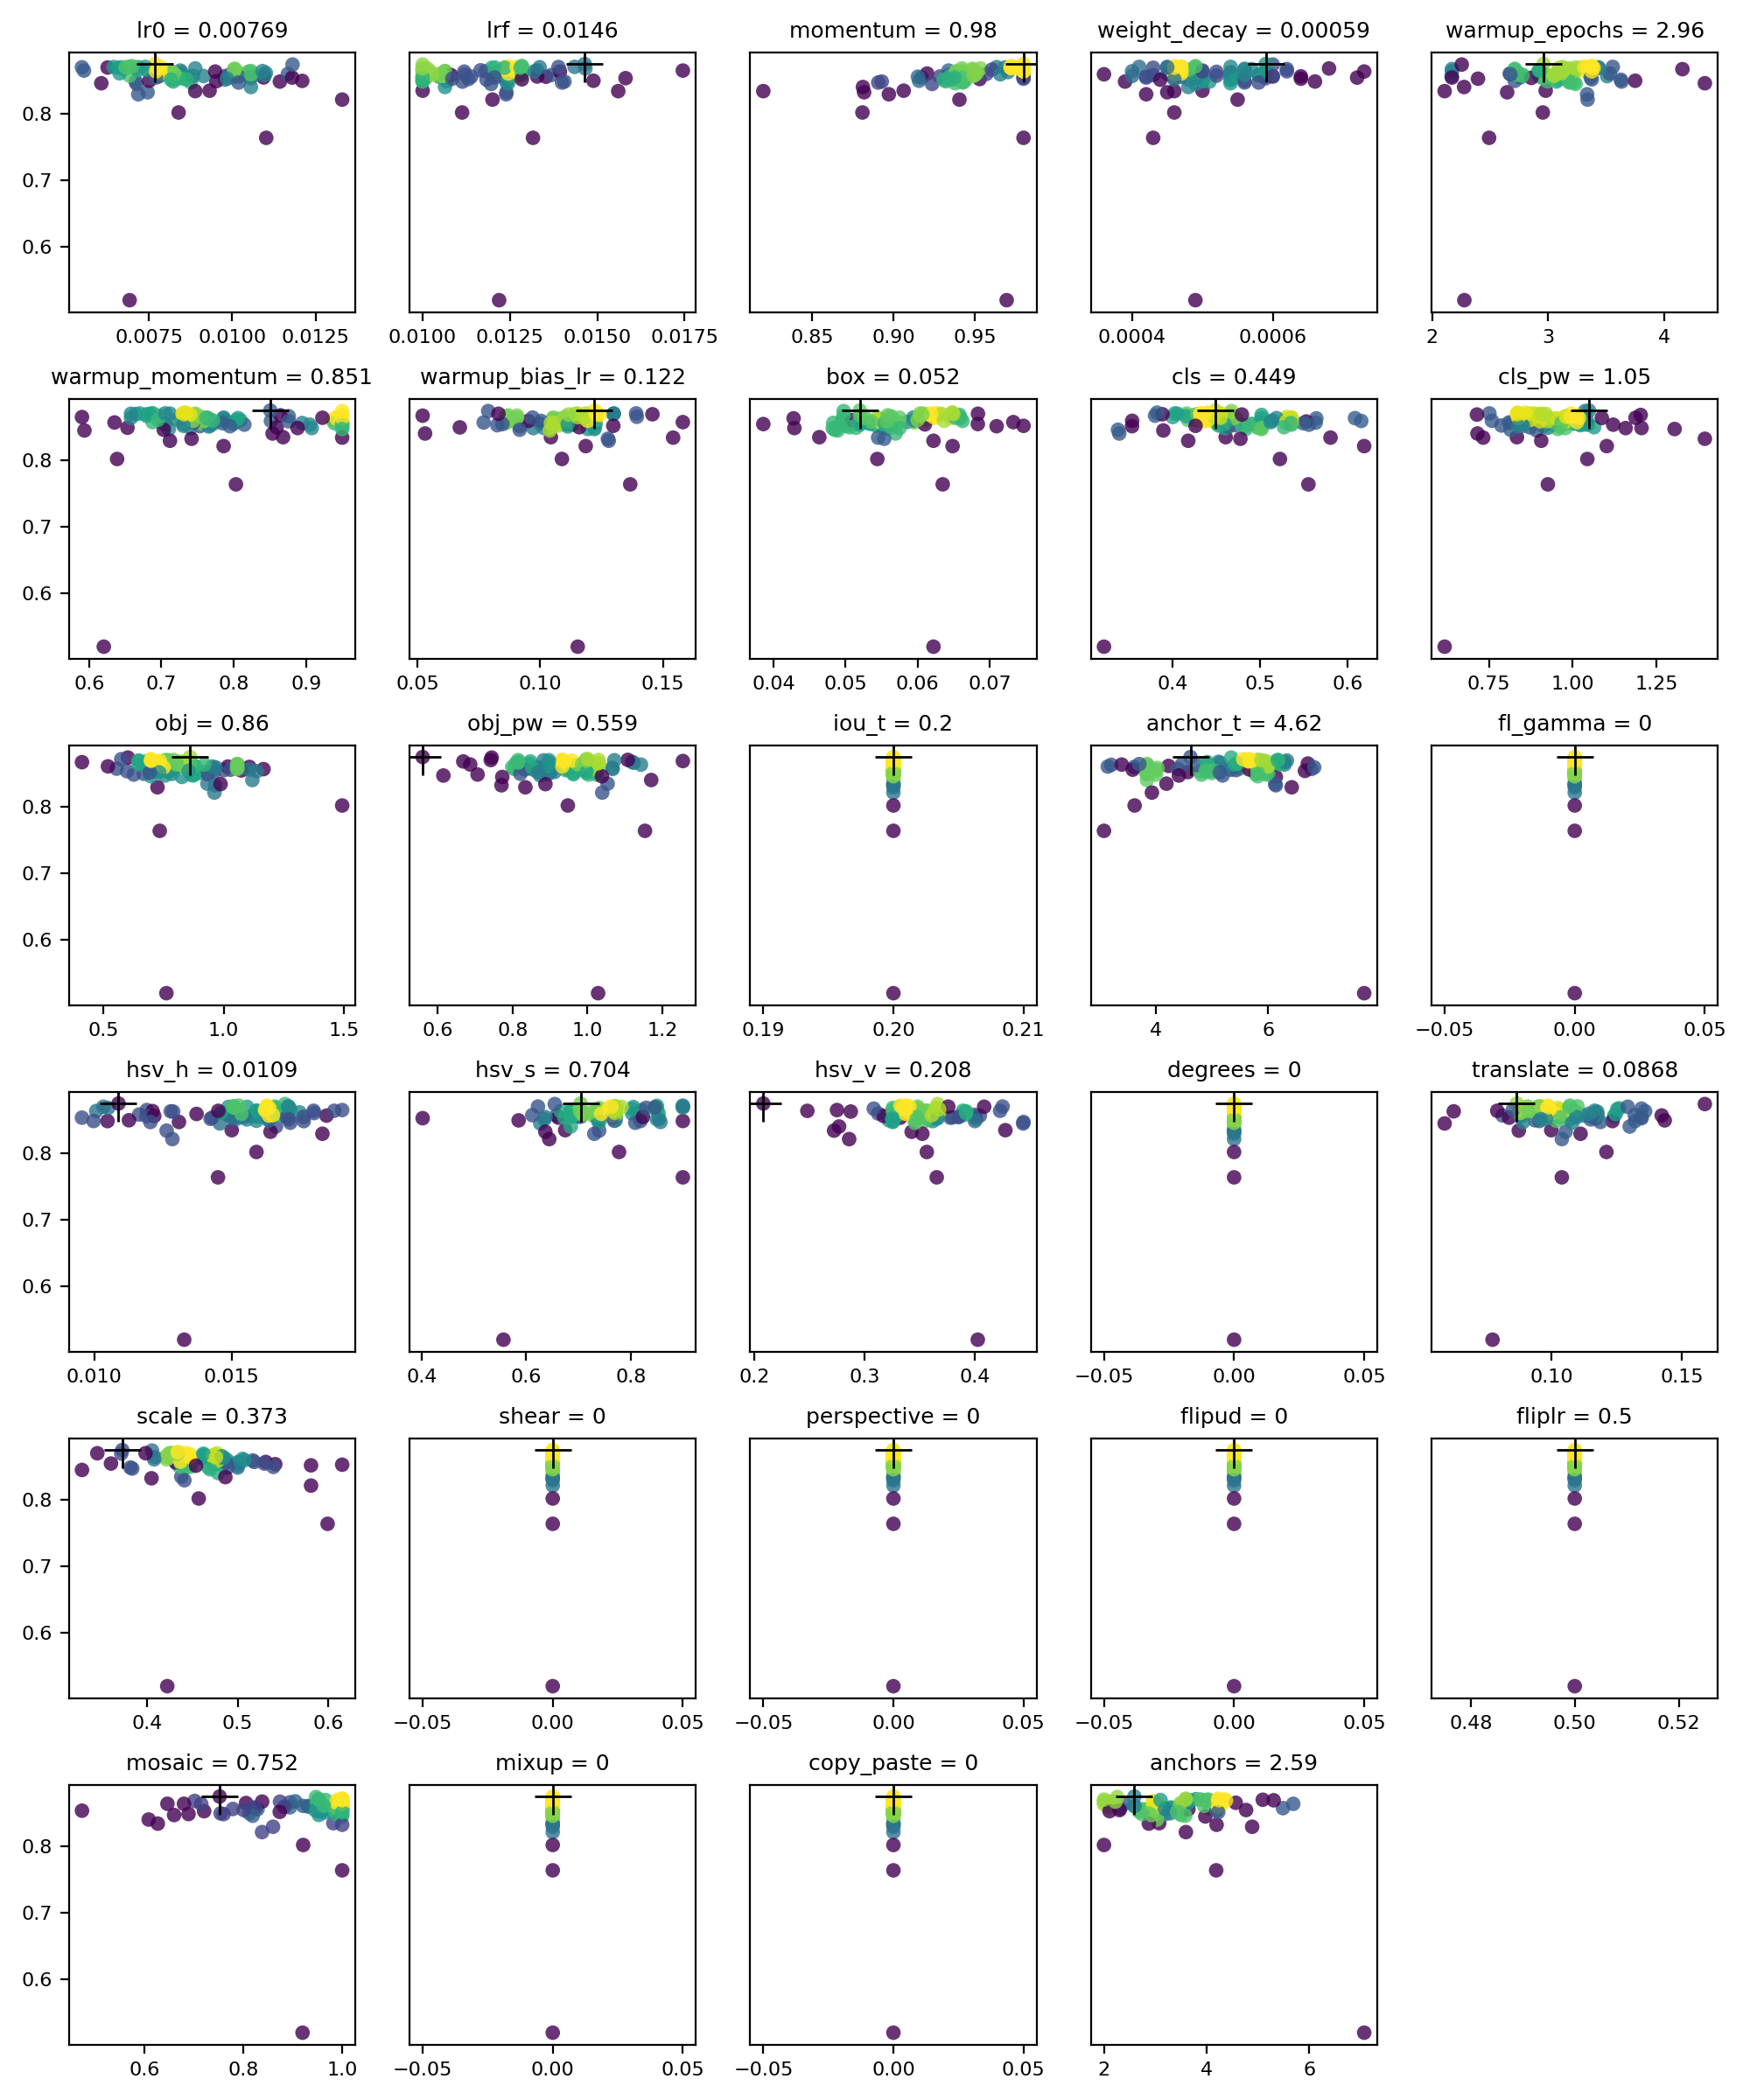
\includegraphics[width=0.8\textwidth]{Sistema de vision artificial/YOLO/evolve_YOLO/evolve.png}
	\caption{Proceso de evolución de los hiperparámetros de YOLO}
	\label{chap:Sistema de visión artificial fig:Evolución YOLO}
\end{figure}

\begin{figure}[H]
	\centering
	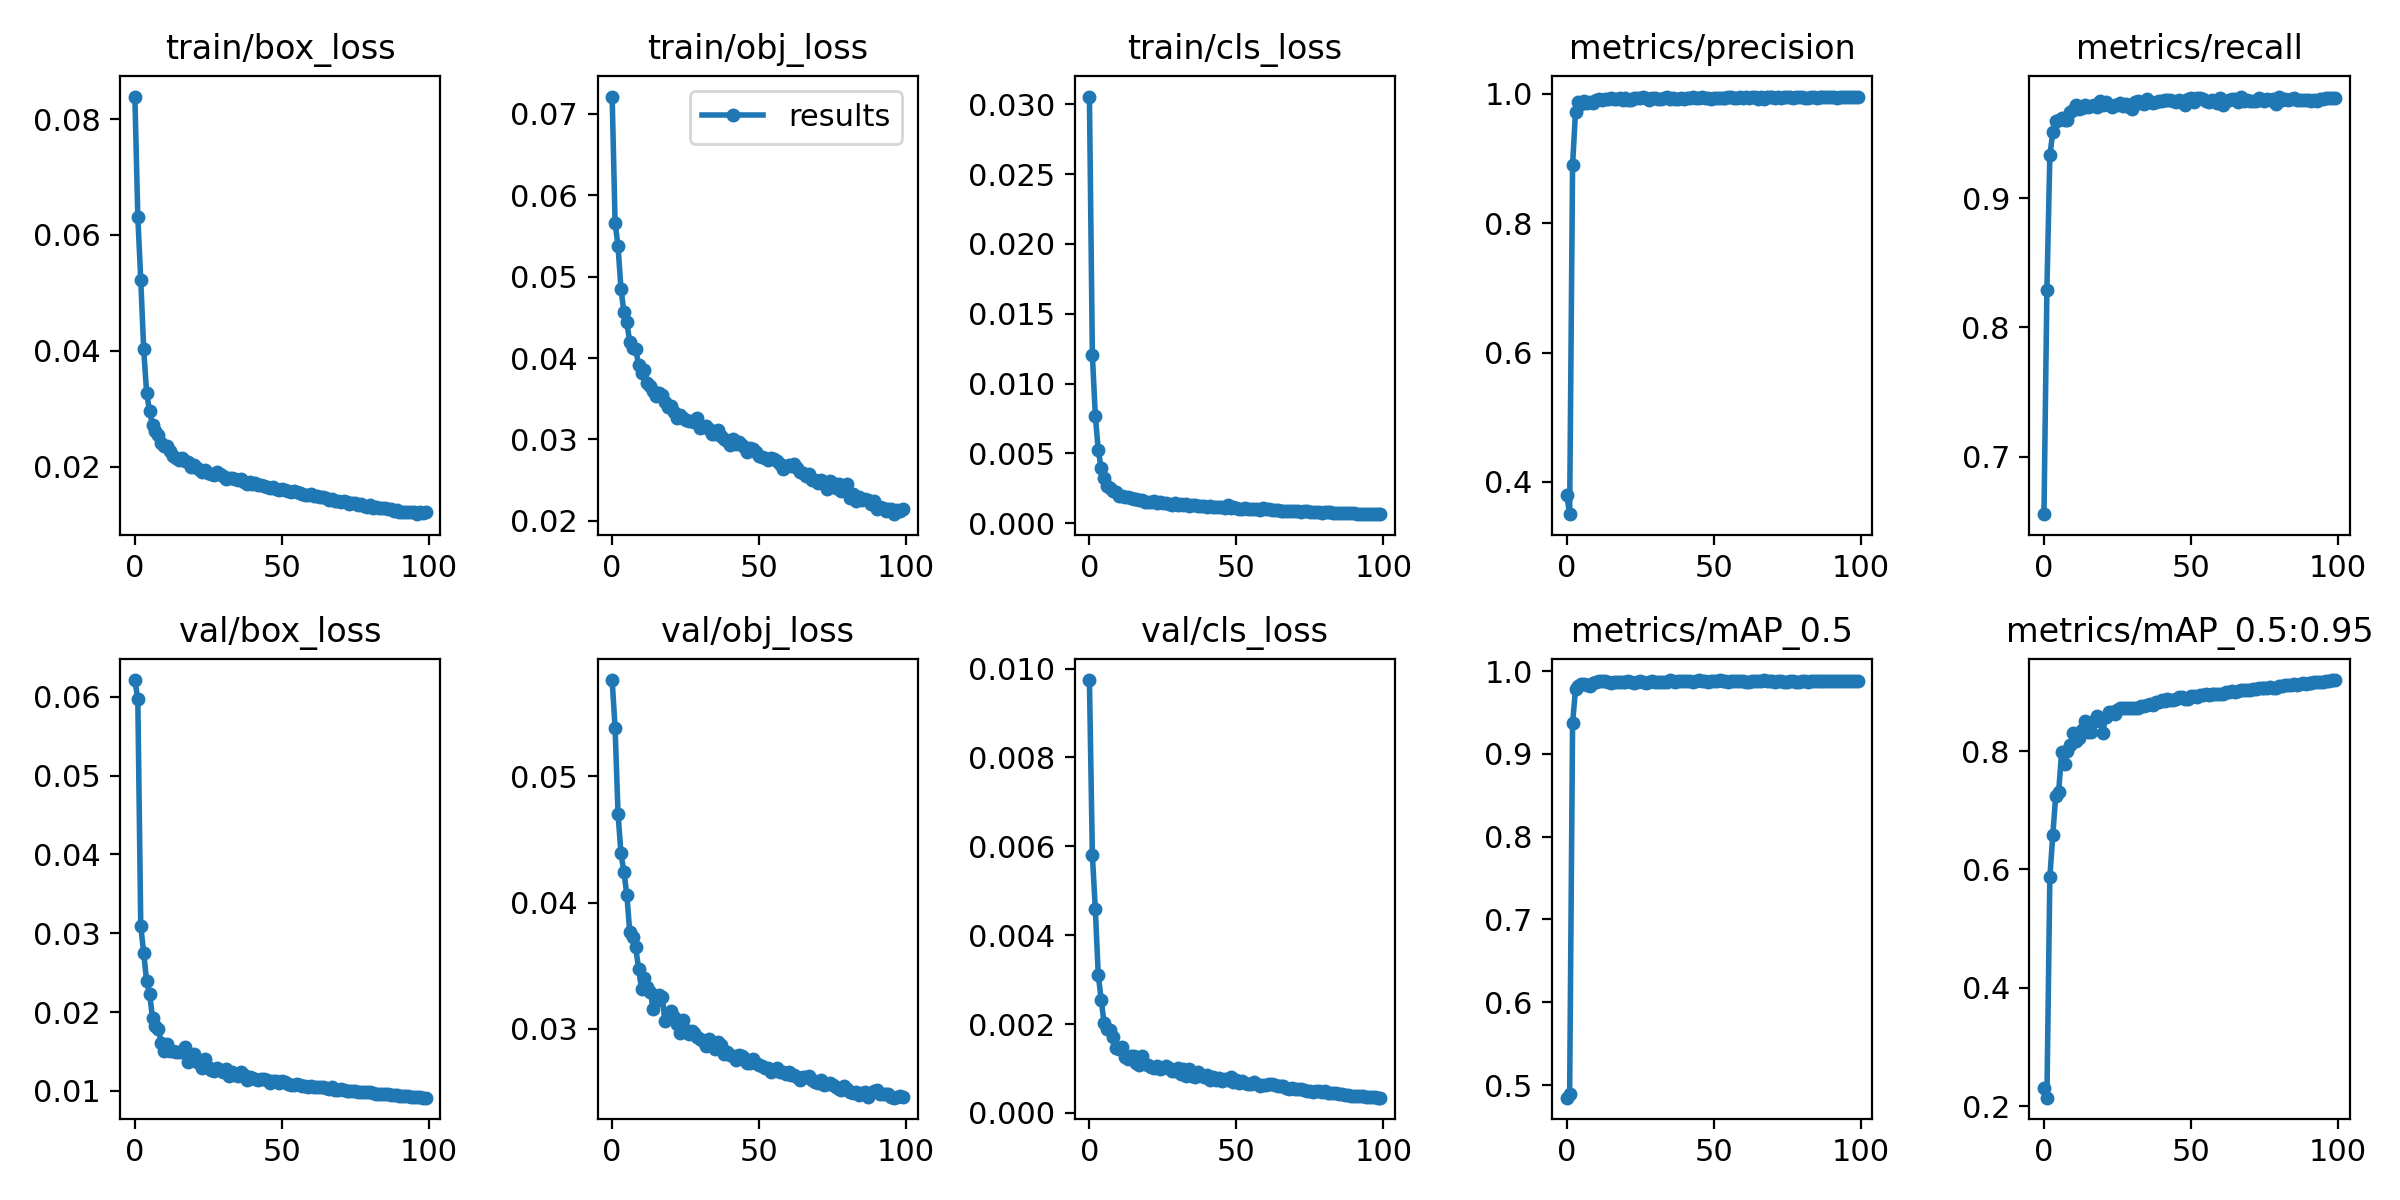
\includegraphics[width=0.8\textwidth]{Sistema de vision artificial/YOLO/evolve_YOLO/results.png}
	\caption{Resultados de la evolución de los hiperparámetros de YOLO}
	\label{chap:Sistema de visión artificial fig:Resultados evolución YOLO}
\end{figure}

\begin{figure}[H]
	\centering
    \includegraphics[width=.32\textwidth]{Sistema de vision artificial/YOLO/metrics_mAP_05_95.png} \hfill
    \includegraphics[width=.32\textwidth]{Sistema de vision artificial/YOLO/metrics_precision.png} \hfill
    \includegraphics[width=.32\textwidth]{Sistema de vision artificial/YOLO/metrics_recall.png}
	\caption[Métricas de la red neuronal YOLO \textit{(mAP 0.5:0.95, precision \& recall)}]{Métricas de la red neuronal YOLO (azul evolutivo y rojo base)}
	\label{chap:Sistema de visión artificial fig:YOLO metrics}
\end{figure}

\begin{figure}[H]
	\centering
    \includegraphics[width=.32\textwidth]{Sistema de vision artificial/YOLO/train_box_loss.png} \hfill
    \includegraphics[width=.32\textwidth]{Sistema de vision artificial/YOLO/train_cls_loss.png} \hfill
    \includegraphics[width=.32\textwidth]{Sistema de vision artificial/YOLO/train_obj_loss.png}
	\caption[Entrenamiento de la red neuronal YOLO \textit{(bounding box loss, class loss \& object loss)}]{Entrenamiento de la red neuronal YOLO (azul evolutivo y rojo base)}
	\label{chap:Sistema de visión artificial fig:YOLO train}
\end{figure}

\begin{figure}[H]
	\centering
    \includegraphics[width=.32\textwidth]{Sistema de vision artificial/YOLO/val_box_loss.png} \hfill
    \includegraphics[width=.32\textwidth]{Sistema de vision artificial/YOLO/val_cls_loss.png} \hfill
    \includegraphics[width=.32\textwidth]{Sistema de vision artificial/YOLO/val_obj_loss.png}
	\caption[Validación de la red neuronal YOLO \textit{(bounding box loss, class loss \& object loss)}]{Validación de la red neuronal YOLO (azul evolutivo y rojo base)}
	\label{chap:Sistema de visión artificial fig:YOLO validation}
\end{figure}

\begin{figure}[H]
	\centering
	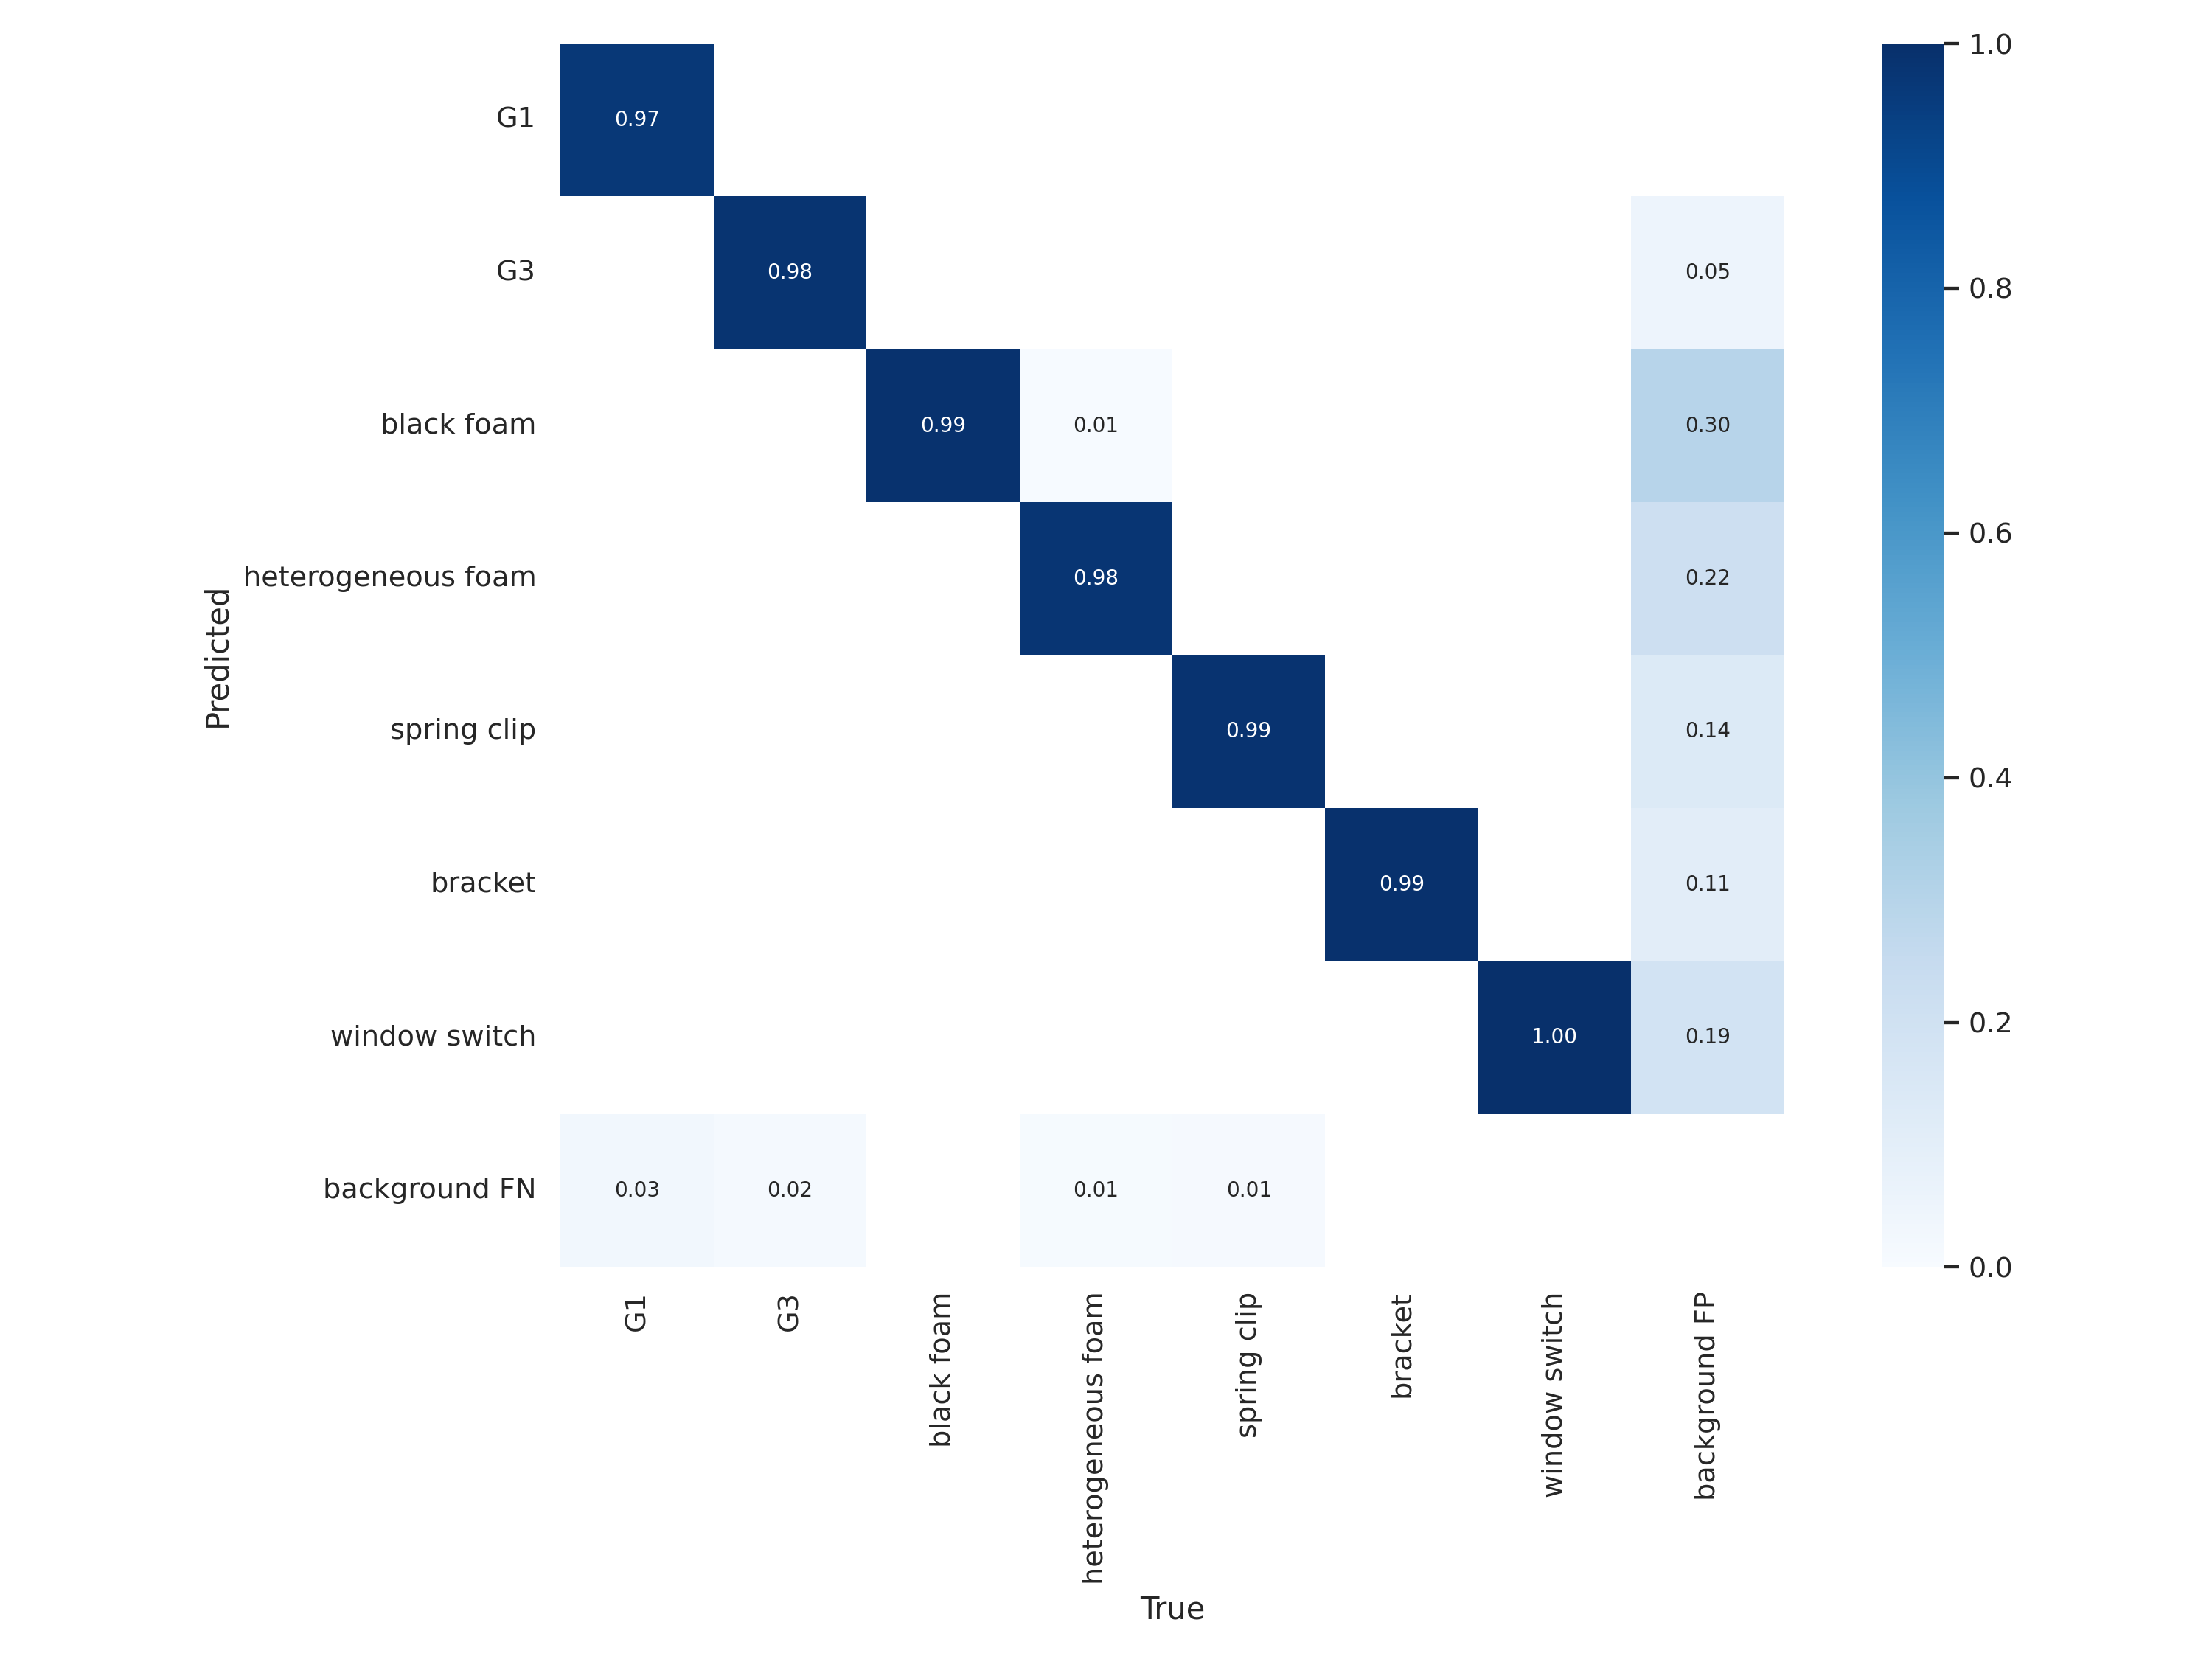
\includegraphics[width=0.8\textwidth]{Sistema de vision artificial/YOLO/Val/confusion_matrix.png}
	\caption{Matriz de confusión en validación de YOLO}
	\label{chap:Sistema de visión artificial fig:YOLO Val Matrix}
\end{figure}

\begin{figure}[H]
	\centering
    \includegraphics[width=0.45\textwidth]{Sistema de vision artificial/YOLO/Val/P_curve.png} \hfill
    \includegraphics[width=0.45\textwidth]{Sistema de vision artificial/YOLO/Val/R_curve.png}
	\caption{\textit{Precision y Recall} en validación de YOLO}
	\label{chap:Sistema de visión artificial fig:YOLO Val PR}
\end{figure}

\begin{figure}[H]
	\centering
	\includegraphics[width=0.5\textwidth]{Sistema de vision artificial/YOLO/Val/F1_curve.png}
	\caption{Curva F1 en validación de YOLO}
	\label{chap:Sistema de visión artificial fig:YOLO Val F1}
\end{figure}

\newpage
\section{Tiny YOLO}
\label{chap:Sistema de visión artificial sec:Tiny YOLO}
Con el fin de determinar los posibles puntos de agarre disponibles en la pieza se ha desarrollado una segunda red neuronal basado en YOLO capaz de detectar dichas regiones. Empleará como entrada un recorte de la pieza detectada por la red neuronal principal y sobre está identificará y detectará aquellos puntos presentes y accesibles. Se emplea una segunda red neuronal debido a que YOLO puede presentar problemas al intentar detectar objetos dentro de objetos debido  la proximidad de los \textit{bounding boxes}. Se deberá de crear y entrenar una red por cada pieza que se desee introducir en el sistema. Esta solución implica un aumento de complejidad al tener que disponer de un gran número de redes pero a su vez permite la creación de un sistema modular capaz de adaptarse a una nueva pieza con rapidez y sin afectar al resto del sistema.

\subsection{Estructura}
\label{chap:Sistema de visión artificial subsec:Tiny YOLO Estructura}
Esta segunda red neuronal se deberá de entrenar tantas veces como piezas de desee introducir al sistema. Es por ello que la carga computacional debe de ser reducida para evitar crear un sistema lento y poco eficiente. Por suerte, debido a la gran especialización de la red, solo debe de detectar regiones para un tipo de pieza, por ello se puede emplear la versión de YOLO de menor tamaño. La principal ventaja de YOLOv5 es el uso de recursos tanto a nivel computacional como de almacenamiento. La red ocupa 4 MB y cuenta con un total de 1.9 millones de neuronas. Pero a pesar de su reducido tamaño es capaz de lograr resultados sorprendentes capaces de competir con potentes y pesadas redes basadas en Fast-RCNN.

\begin{figure}[ht]
	\centering
	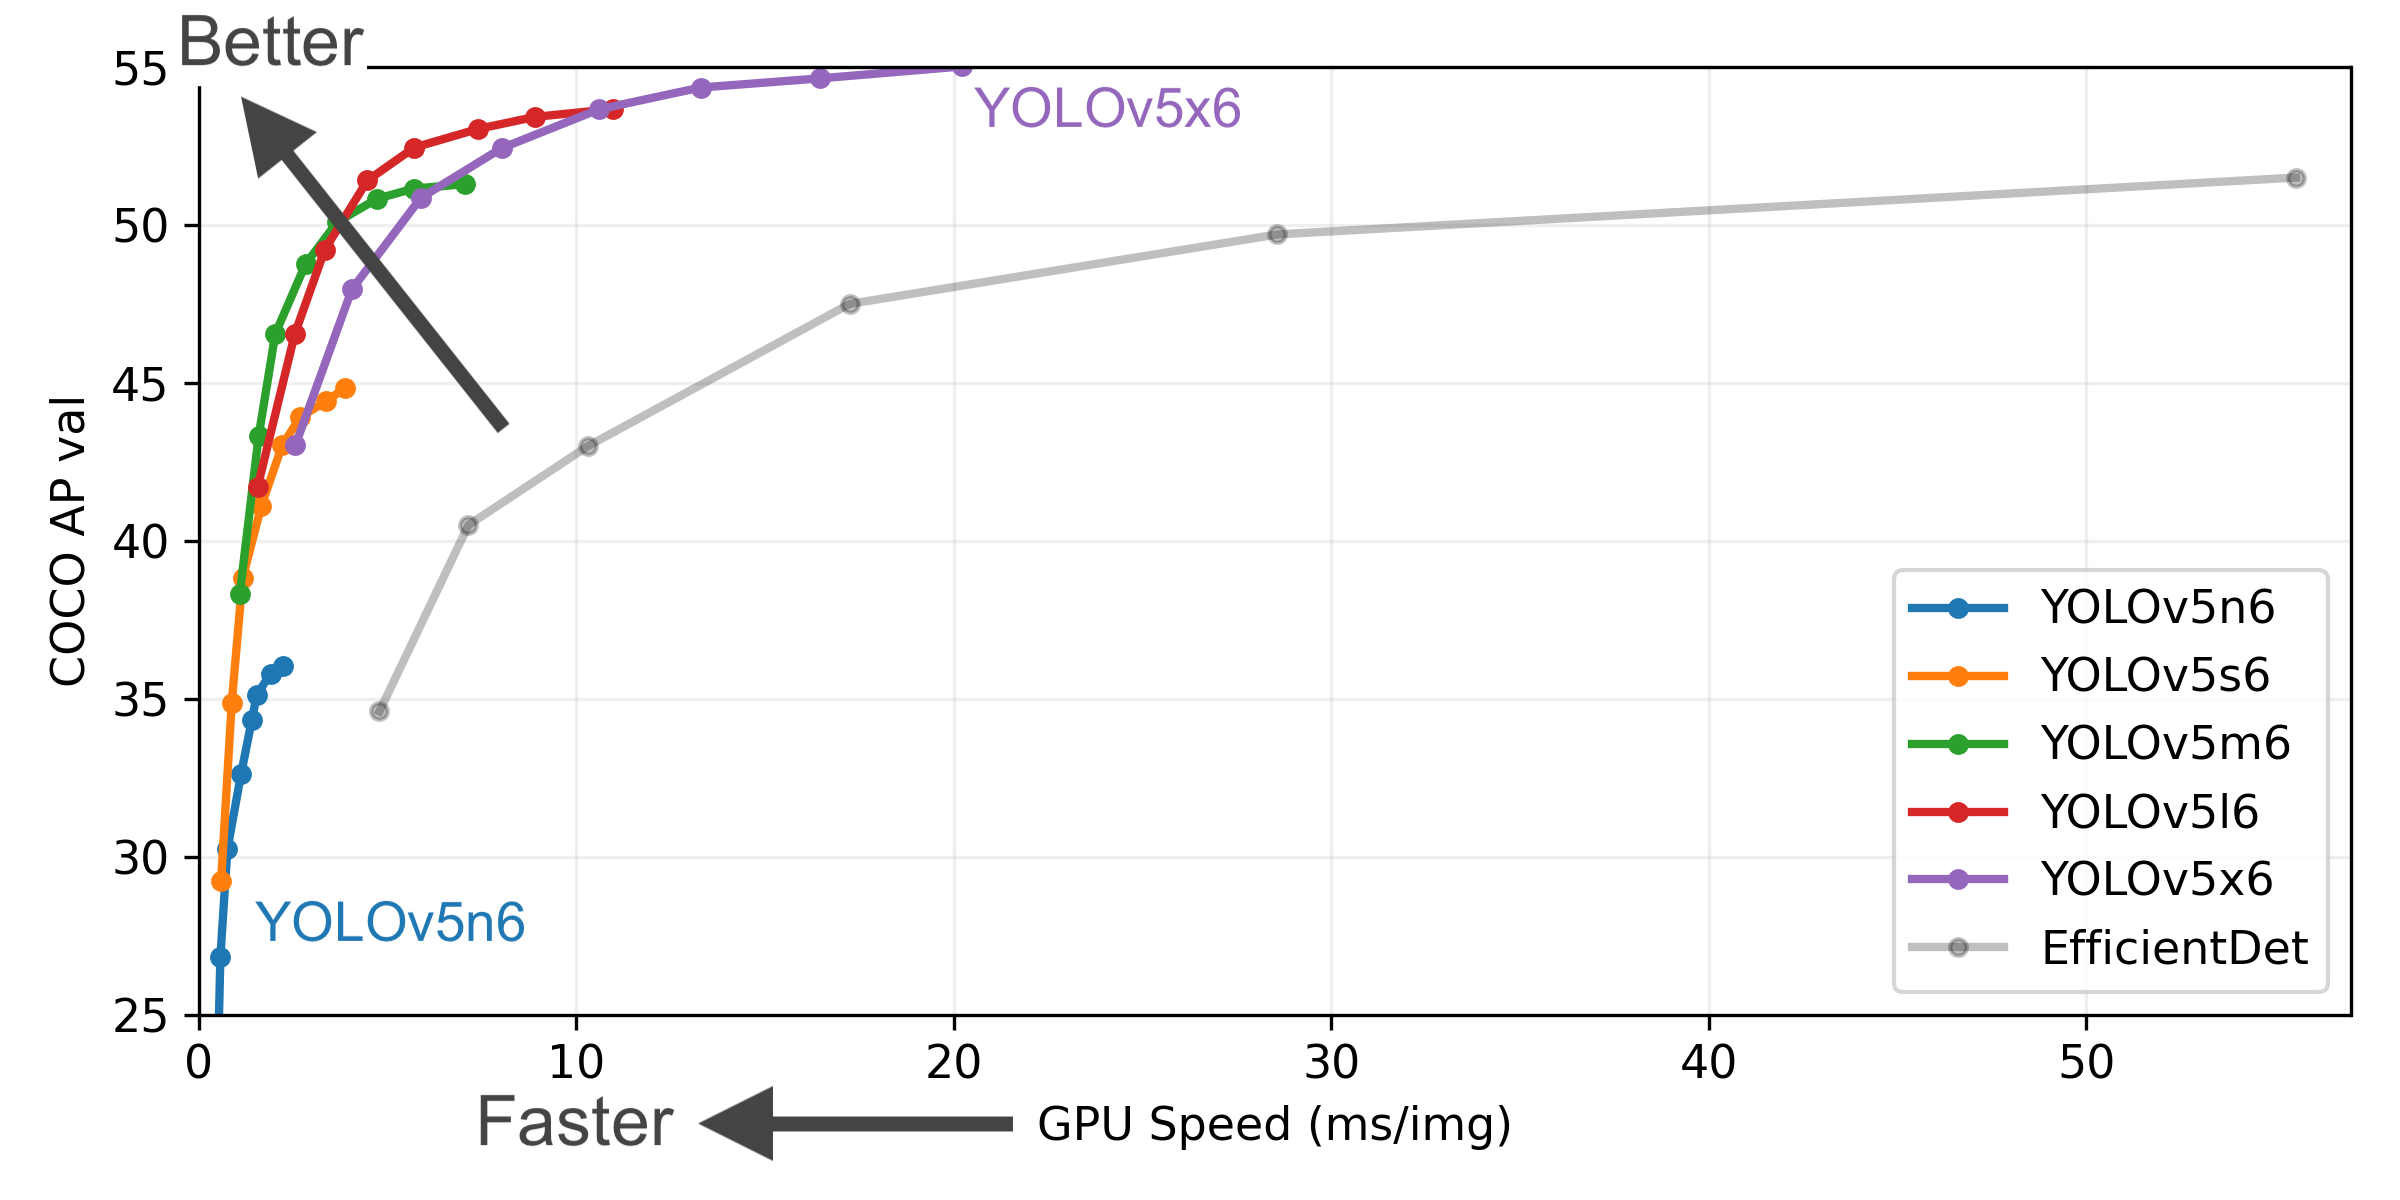
\includegraphics[width=0.7\textwidth]{Sistema de vision artificial/YOLO/comparativa_YOLO.png}
	\caption{Comparativa de los diferentes modelos de YOLO}
	\label{chap:Sistema de visión artificial fig:Comparativa YOLO}
\end{figure}

\subsection{Entrenamiento}
\label{chap:Sistema de visión artificial sec:Tiny YOLO Entrenamiento}
Como se ha visto anteriormente, una de las mejoras introducidas en YOLOV5 consiste en la optimización de los hiperparámetros de forma autónoma empleando un algoritmo genético. Sin embargo, este tipo de entrenamiento aumenta significativamente la carga computacional necesaria ya que se debe de entrenar múltiples veces la misma red para determinar la configuración óptima. En el caso de la red principal este es un gasto asumible ya que solo se deberá de entrenar una red. Para la red secundaria se debe de entrenar un modelo para cada pieza. Es por ello que con el fin de reducir los tiempos de entrenamiento se empleará los hiperparámetros obtenidos por el proceso evolutivo de la red YOLO.

\begin{table}[ht]
  \centering
    \begin{tabular}{|c|c|}
    \hline
    \multicolumn{2}{|c|}{Opciones de entrenamiento} \\
    \hline
    Parametro & Valor \\
    \hline
    Optimizador & SGD momentum/Adam betal \\
    \hline
    Initial learn rate & 0.00769 \\
    \hline
    Learn rate decay & 0.01464 \\
    \hline
    Momentum & 0.98 \\
    \hline
    Weight decay & 0.00059 \\
    \hline
    Warmup epochs & 2.961 \\
    \hline
    Warmup momentun & 0.85061 \\
    \hline
    Box loss gain & 0.05199 \\
    \hline
    CLS loss gain & 0.4489 \\
    \hline
    IoU threshold & 0.2 \\
    \hline
    Anchor threshold & 4.6172 \\
    \hline
    Epochs & 250 \\
    \hline
    Batch Size & 96 \\
    \hline
    \end{tabular}
  \caption{Opciones de entrenamiento de TINY YOLO}
  \label{chap:Sistema de visión artificial tab:TINY YOLO options}
\end{table}

\subsection{Resultados}
\label{chap:Sistema de visión artificial sec:Tiny YOLO Resultados}
Tiny YOLO debe de ser entrenado tantas veces como piezas grandes haya presentes en el sistema.Por lo cual se ha tenido que entrenar múltiples veces y se dispone de numerosas redes y resultados. pero con el fin de simplificar este documento y para evitar redundancia solo se va a mostrar el proceso de entrenamiento y los resultados de una pieza. La pieza seleccionada es G1 y consta de un total de 5 posibles puntos de agarre.

Con la ayuda de YOLO se ha podido realizar un último análisis del \textit{dataset} empleado con el fin de determinar las instancias, la ubicación y forma de los diferentes puntos presentes. Y determinar si existe alguna correlación entre estos y patrones en la distribución de piezas. Al analizar los resultados mostrados en la \autoref{chap:Sistema de visión artificial fig:TINY YOLO labels} se observa a simple vista múltiples patrones tanto en distribución como en forma de las piezas a detectar. Para entender estos patrones es necesario entender que se está intentando detectar, se desea identificar regiones con puntos de agarre dentro de una pieza y en este caso nos estamos centrando en la pieza G1. Estas regiones se han definido con la ayuda de códigos QR basados en la tecnología Aruco implantados dentro de la geometría 3D de la pieza. Esto implica que en todas las piezas los códigos se encuentran siempre en las mismas posiciones y dimensiones relativas a la pieza. Por ello se pueden observar los siguientes patrones:

\begin{itemize}
\item Instancias: Se observa una mayor número ed instancias del punto 5. Esto se debe al comportamiento de la pieza G1 y su tendencia a acabar en posiciones determinadas.
\item Posición: se observa un patrón con forma de estrella que representa las zonas con un mayor número de instancias. Esta geometría se debe al elevado tamaño e la pieza G1 respecto a la zona de trabajo. Debido a las dimensiones esta pieza presenta posiciones con una alta ocurrencia.
\item Tamaño: al enfrentar el ancho y alto de las instancias destaca una clara proporción 1:1 entre estas. Esto se debe a que los códigos QR empleados son cuadrados.
\end{itemize}

Se recomiendo replantear la configuración del generador de imágenes para adaptar el entorno de trabajo a la pieza con el objetivo de evitar la presencia de posiciones frecuentes. Esto se puede realizar con la inclusión de nuevos entornos de trabajo que añadan riqueza y aleatoriedad.
	

\begin{figure}[ht]
  \subfloat{
	\begin{minipage}[c][1\width]{0.49\textwidth}
	   \centering
	   \includegraphics[width=1\textwidth]{Sistema de vision artificial/TINY YOLO/Train/labels.jpg}
	\end{minipage}}
  \hfill	
  \subfloat{
	\begin{minipage}[c][1\width]{0.49\textwidth}
	   \centering
	   \includegraphics[width=1\textwidth]{Sistema de vision artificial/TINY YOLO/Train/labels_correlogram.jpg}
	\end{minipage}}
\caption{Evaluación de instancias, forma y ubicación del \textit{dataset} basado en G1 empleado en TINY YOLO}
\label{chap:Sistema de visión artificial fig:TINY YOLO labels}
\end{figure}

Tras entrenar durante un total de 250 \textit{epochs} se puede observar que la red neuronal ha conseguido aprender, extraer y generalizar la información disponible en el \textit{dataset}.Con lo que se ha podido reducir drásticamente las perdidas (\textit{object, class \& box}) tanto en entrenamiento como en validación. En este entrenamiento se puede apreciar que a pesar de ser un caso más simple, con un a red de menor tamaño y un mayor número de \textit{epochs}, la red todavía presenta un margen de mejora. El error en validación todavía presenta una tendencia decreciente cuando se detuvo el entrenamiento. El motivo de no continuar con el entrenamiento son limitaciones de tiempo y carga computacional.

Por último, se ha obtenido la precision y el \textit{recall} de validación (ver \autoref{chap:Sistema de visión artificial fig:TINY YOLO Val PR}). Con la precisión se observa como con un nivel de confianza del 80\% se pueden obtener resultados con una precisión elevada y similares a la red YOLO con un nivel de confianza del 40\%. Esta reducción de precision frente a YOLO se puede deber a varios factores:

\begin{itemize}
\item Red: al emplear la version yolov5n se reduce de forma considerable las capacidades de la red.
\item Tipo de pieza a detectar: en este caso se desea detectar regiones de interés dentro de una pieza. Es decir, estas no presentan un borde claro que se pueda distinguir frente al fondo. Esto puede afectar en gran medida a la red que se ve incapaz de determinar los limites del objeto a detectar.
\item Tamaño de la pieza: todas las instancias empleadas en este entrenamiento han sido diseñadas por ordenador y presentan unas dimensiones exactas. Esto puede sesgar las capacidades del sistema y puede llevarlo a realizar asunciones.
\end{itemize}

Y con \textit{recall} se observa como ha medida que aumentamos el nivel de confianza requerido aumenta el numero de falsos negativos (piezas no detectadas). En la curva F1 se enfrentan ambas métricas permitiendo ver de forma visual como afecta el nivel de confianza a la identificación de piezas. Se observa como el modelo final debe de trabajar con un nivel de confianza entre el 40\% y 80\% para obtener resultados óptimos.

\begin{figure}[H]
	\centering
    \includegraphics[width=.32\textwidth]{Sistema de vision artificial/TINY YOLO/metrics_mAP_05_95.png} \hfill
    \includegraphics[width=.32\textwidth]{Sistema de vision artificial/TINY YOLO/metrics_precision.png} \hfill
    \includegraphics[width=.32\textwidth]{Sistema de vision artificial/TINY YOLO/metrics_recall.png}
	\caption[Métricas de la red neuronal TINY YOLO \textit{(mAP 0.5:0.95, precision \& recall)}]{Métricas de la red neuronal TINY YOLO (azul evolutivo y rojo base)}
	\label{chap:Sistema de visión artificial fig:TINY YOLO metrics}
\end{figure}

\begin{figure}[H]
	\centering
    \includegraphics[width=.32\textwidth]{Sistema de vision artificial/TINY YOLO/train_box_loss.png} \hfill
    \includegraphics[width=.32\textwidth]{Sistema de vision artificial/TINY YOLO/train_cls_loss.png} \hfill
    \includegraphics[width=.32\textwidth]{Sistema de vision artificial/TINY YOLO/train_obj_loss.png}
	\caption[Entrenamiento de la red neuronal TINY YOLO \textit{(bounding box loss, class loss \& object loss)}]{Entrenamiento de la red neuronal TINY YOLO (azul evolutivo y rojo base)}
	\label{chap:Sistema de visión artificial fig:TINY YOLO train}
\end{figure}

\begin{figure}[H]
	\centering
    \includegraphics[width=.32\textwidth]{Sistema de vision artificial/TINY YOLO/val_box_loss.png} \hfill
    \includegraphics[width=.32\textwidth]{Sistema de vision artificial/TINY YOLO/val_cls_loss.png} \hfill
    \includegraphics[width=.32\textwidth]{Sistema de vision artificial/TINY YOLO/val_obj_loss.png}
	\caption[Validación de la red neuronal TINY YOLO \textit{(bounding box loss, class loss \& object loss)}]{Validación de la red neuronal TINY YOLO (azul evolutivo y rojo base)}
	\label{chap:Sistema de visión artificial fig:TINY YOLO validation}
\end{figure}

\begin{figure}[H]
	\centering
	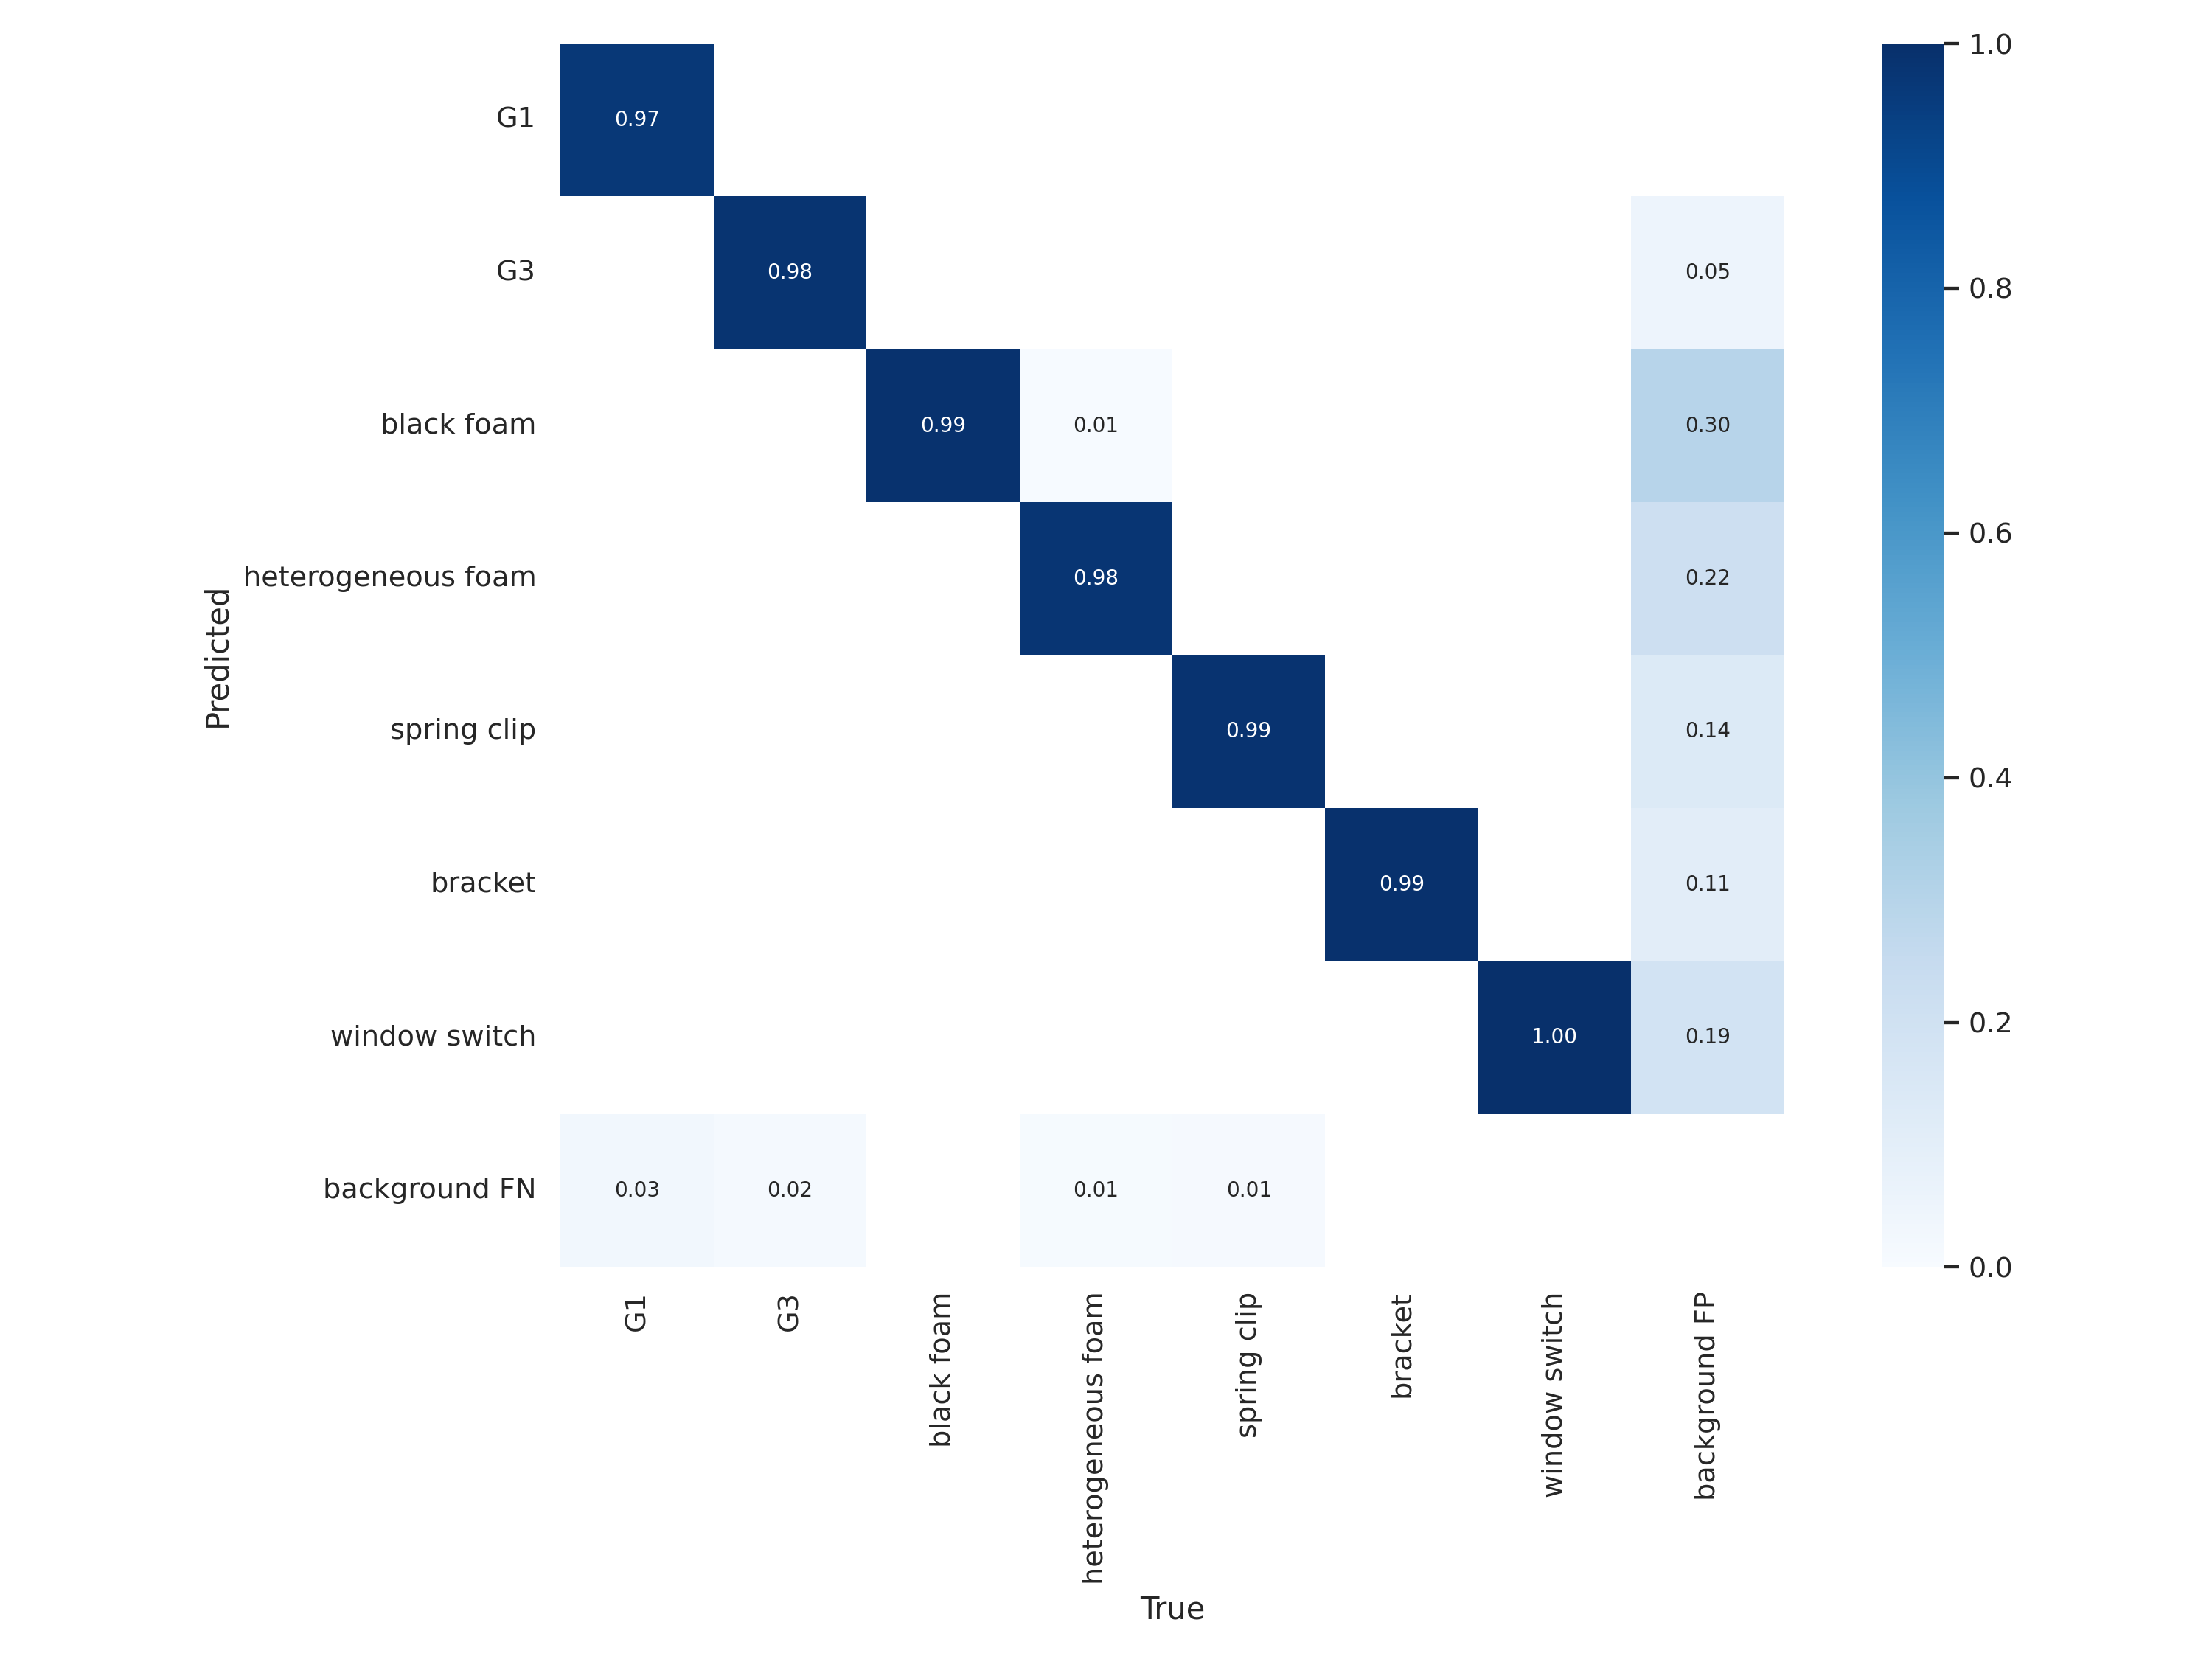
\includegraphics[width=0.8\textwidth]{Sistema de vision artificial/YOLO/Val/confusion_matrix.png}
	\caption{Matriz de confusión en validación de TINY YOLO}
	\label{chap:Sistema de visión artificial fig:TINY YOLO Val Matrix}
\end{figure}

\begin{figure}[H]
	\centering
    \includegraphics[width=0.45\textwidth]{Sistema de vision artificial/TINY YOLO/Val/P_curve.png} \hfill
    \includegraphics[width=0.45\textwidth]{Sistema de vision artificial/TINY YOLO/Val/R_curve.png}
	\caption{\textit{Precision y Recall} en validación de TINY YOLO}
	\label{chap:Sistema de visión artificial fig:TINY YOLO Val PR}
\end{figure}

\begin{figure}[H]
	\centering
	\includegraphics[width=0.5\textwidth]{Sistema de vision artificial/TINY YOLO/Val/F1_curve.png}
	\caption{Curva F1 en validación de TINY YOLO}
	\label{chap:Sistema de visión artificial fig:TINY YOLO Val F1}
\end{figure}


\newpage
\section{Regresor}
\label{chap:Sistema de visión artificial sec:Regresor}
Los últimos elementos necesarios para poder agarrar la pieza deseada es la determinación del punto de agarre óptimo y el vector normal a dicho punto. Gracias a la red neuronal TINY YOLO es posible determinar el punto óptimo pero se todavía se desconoce con precisión sus coordenadas. Por ello se ha introducido una tercera red neuronal encargada de determinar las cinco coordenadas necesarias (x, y, u,v y w).

Para simplificar el proceso lo máximo posible, esta última capa se entrenará de forma individual para cada posible punto de agarre. Esto implica que se dispondrán de tantos pesos como puntos de agarre. Esta red empleará como entrada un recorte de la pieza detectada por la red neuronal principal. Esta solución implica un aumento de complejidad al tener que disponer de un gran número de redes pero a su vez permite la creación de un sistema modular capaz de adaptarse a un cambio en la pieza con rapidez y sin afectar al resto del sistema. Además se permite reducir la carga sobre la red al simplificar el proceso lo máximo posible.

\subsection{Estructura}
\label{chap:Sistema de visión artificial subsec:Regresor Estructura}
Esta tercera red neuronal se deberá de entrenar tantas veces como puntos de desee introducir al sistema. Es por ello que la carga computacional debe de ser reducida para evitar crear un sistema lento y poco eficiente. Pero tampoco se desea crear un sistema incapaz de extraer las características de la pieza y determinar los puntos de agarre. Teniendo esto en cuenta se ha desarrollado una red neuronal dividida en dos secciones, una primera sección basada en la convolución y encargada de extraer las características de la pieza. Y una segunda sección del tipo \textit{fully connected} basada en perceptrones que se encargarán de analizar las características extraídas por las primeras capas. En base a estas estimarán las coordenadas del punto de agarre.

El desarrollo de una red neuronal es un proceso laborioso que requiere de múltiples pruebas e intentos con el fin de conseguir desarrollar un sistema que aprenda y de forma optimizada. Es por ello por lo que se han tenido que desarrollar y entrenar múltiples redes para dar con un sistema óptimo. El primer paso en el desarrollo de la red ha sido comparar el impacto de diferentes tamaños de redes. Se han comparado redes con tres, cinco y siete capas convolucionales para determinar el número de capas necesarias para poder extraer las características. Como se verá en las secciones de entrenamientos y resultados, de estas pruebas se ha determina que un número de capas óptimo en base a la fase de entrenamiento es cinco. Sin embargo, estos resultados varían drásticamente cuando se analiza los resultados de validación. En esta última fase se observa mejores resultados con la red neuronal del el máximo número de capas de convolución. Se puede plantear un aumento del número de capas para mejorar los resultados pero esto a su vez implica un aumento de carga computacional. Por ello se ha optado por fijar el número de capas convolucionales en siete. Las capas estan constituidas por un conjunto de capa convolucional seguida por una capa de normalización y finalmente una capa de activación tipo SiLu.

A la vez que se comprobó el impacto del número de capas de convolución, se comprobó el impacto del tamaño del regresor. Y se obtuvieron resultados similares a las capas de convolución. Se desarrollaron redes con dos, tres y cuatro redes de convolución y se obtuvo que mejores resultados con un sistema constituido por cinco capas del tipo \textit{fully connected}.

Una vez establecido el número de capas se determino el impacto de diferentes funciones de activación (ReLu frente a SiLu) y se comparó diferentes criterios para la determinación del error (L1Loss frente a MSELoss) y diferentes optimizadores (Adam frente a SGD). De todas estas pruebas (visibles en el apartado de entrenamiento) se determino que los mejores resultados se obtuvieron con la capa de activación SiLu, el criterio L1Loss y el optimizador Adam.

Finalmente se comprobó el impacto de una capa del tipo \textit{Dropout} debido a que se observaba una gran diferencia de resultados entre entrenamiento y validación. Se comprobó el impacto de una capa entre el proceso de convolución y el regresor. Y también se comprobó el impacto de una capa \textit{Dropout} dentro del regresor. En ambos casos se entrenó para diferentes valores de \textit{Dropout} (0.1, 0.3 y 0.5) y en los seis entrenamientos se obtuvo peores resultados frente a la red sin capa \textit{Dropout}. Es por ello por lo que se excluyo de la red.

Tras analizar todos los resultados se determinó que la tercera red del proceso en un sistema constituido por siete capas de convolución y cuatro del tipo \textit{fully connected}. Estas capas a su vez son activadas por la función SiLu y no se empleará ninguna capa del tipo \textit{Dropout}.


\begin{figure}[ht]
	\centering
	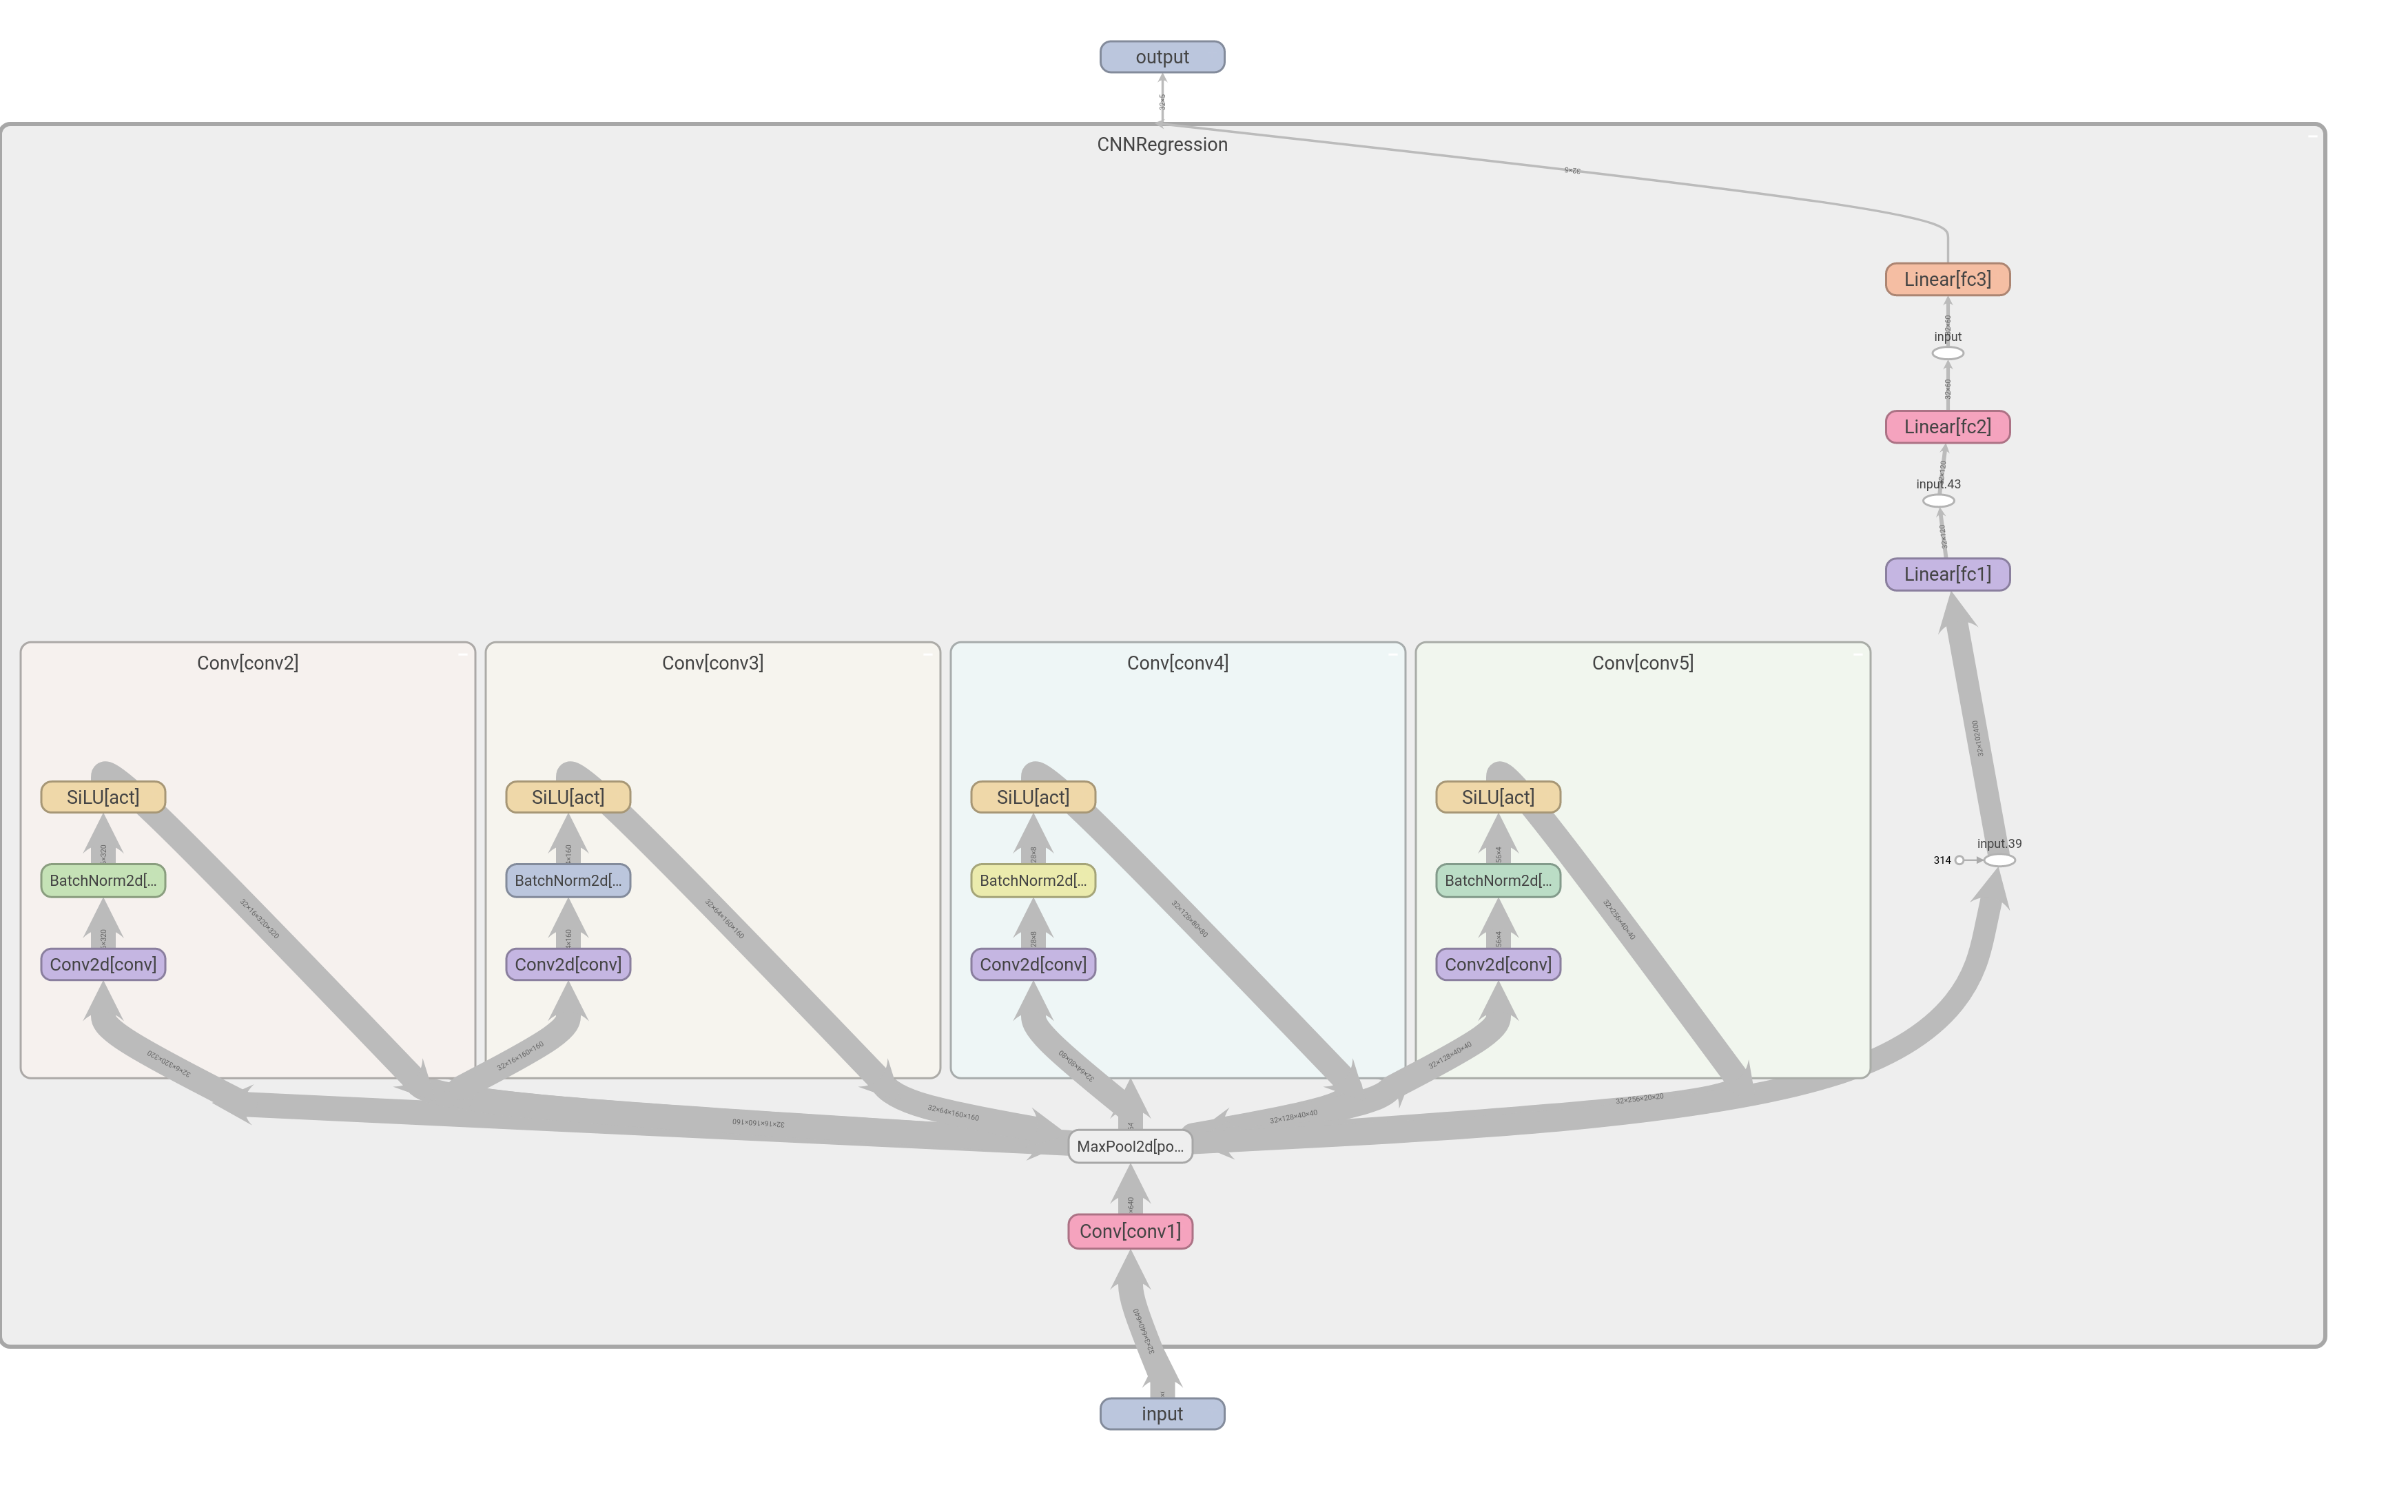
\includegraphics[width=0.7\textwidth]{Sistema de vision artificial/REGRESSION/CNNRegression.png}
	\caption{Estructura del regresor}
	\label{chap:Sistema de visión artificial fig:Estructura Regresor}
\end{figure}

\subsection{Entrenamiento}
\label{chap:Sistema de visión artificial sec:Regresor Entrenamiento}
Debido al gran número de veces que se deberá de entrenar esta red neuronal, tantas como puntos de agarre por cada pieza. Se ha fijado como objetivo reducir la carga computacional en la medida de lo posible. Esto implica que el tamaño de la red debe de ser reducido y el número de \textit{epochs} debe de ser limitado a 100. Con este objetivo en mente se ha desarrollado la siguiente configuración para el entrenamiento.

\begin{table}[ht]
  \centering
    \begin{tabular}{|c|c|}
    \hline
    \multicolumn{2}{|c|}{Opciones de entrenamiento} \\
    \hline
    Parametro & Valor \\
    \hline
    Optimizador & Adam \\
    \hline
    Criterio & L1loss \\
    \hline
    Initial learn rate & 1e-04 \\
    \hline
    Learn rate decay & 0.5 \\
    \hline
    Learn rate step & 15 \\
    \hline
    Epochs & 100 \\
    \hline
    Batch Size & 32 \\
    \hline
    \end{tabular}
  \caption{Opciones de entrenamiento de Regresor}
  \label{chap:Sistema de visión artificial tab:Regresor options}
\end{table}


\subsection{Resultados}
\label{chap:Sistema de visión artificial sec:Regresor Resultados}
El regresor debe de ser tantas veces como puntos en cada pieza grande haya. Es por esto que la red y el entrenamiento se han visto limitados. A pesar de esta limitación se han conseguido resultados que demuestran las capacidades del sistema a la hora de determinar los puntos de agarre. En estos resultados se muestra el impacto de las diferentes tipos de redes desarrolladas.

Destaca con los mejores resultados la red con el mayor número de capas de convolución y sin capas \textit{Dropout}. Y con este tipo de red se consigue obtener un error entorno al 5\% en validación para los vectores normales y entorno al 1-2\% para la determinación del punto de agarre. También destaca en esta red los errores de validación de los vectores normales donde a pesar del entrenamiento se dan situaciones en donde los resultados obtenidos empeoran al aumentar el entrenamiento. Esto se debe a una combinación de sobreaprendizaje junto un la utilización de un \textit{dataset} sesgado. Esto conlleva a la red a asumir las posiciones de los vectores normales y es por ello por lo que aumenta el error total a pesar del entrenamiento. Se intentó solventar el problema con la utilización de una capa \textit{dropout} pero esta afecto negativamente a rendimiento del sistema ya que le problema reside en una mayor medida en el \textit{dataset}. Si se desean mejorar los resultados se debe de evitar el sesgado antes de intentar mejorar la red. 

\begin{figure}[ht]
\centering
\begin{tabular}{cc}
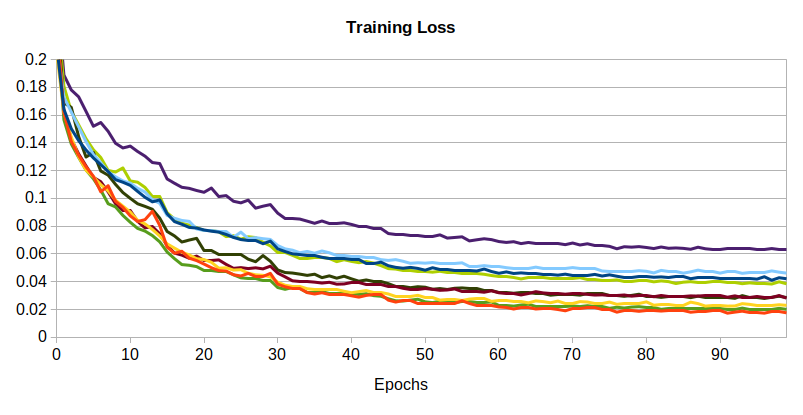
\includegraphics[width=0.45\textwidth]{Sistema de vision artificial/REGRESSION/train_loss.png} &
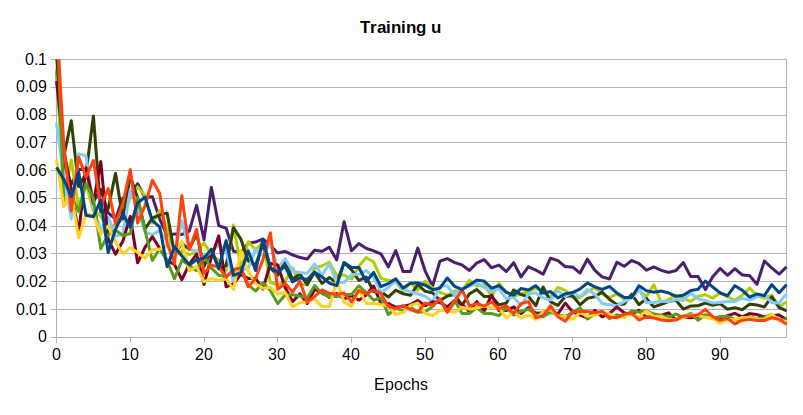
\includegraphics[width=0.45\textwidth]{Sistema de vision artificial/REGRESSION/train_u.png}
\end{tabular}
\begin{tabular}{cc}
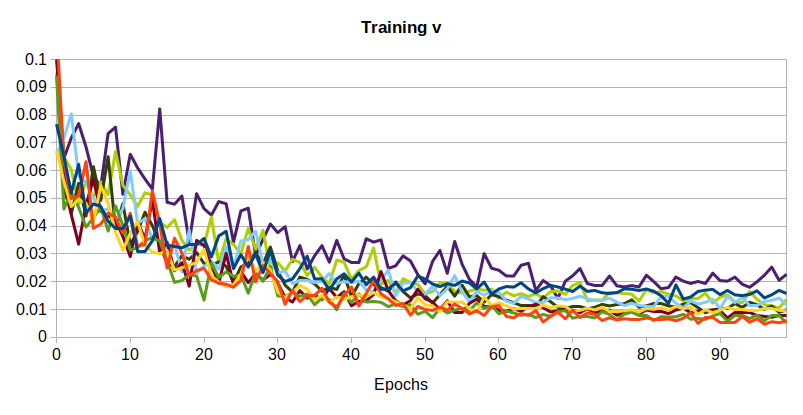
\includegraphics[width=0.45\textwidth]{Sistema de vision artificial/REGRESSION/train_v.png} &
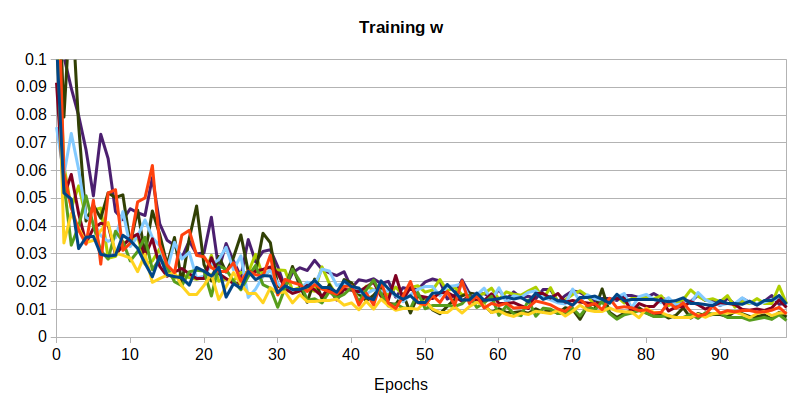
\includegraphics[width=0.45\textwidth]{Sistema de vision artificial/REGRESSION/train_w.png}
\end{tabular}
\begin{tabular}{cc}
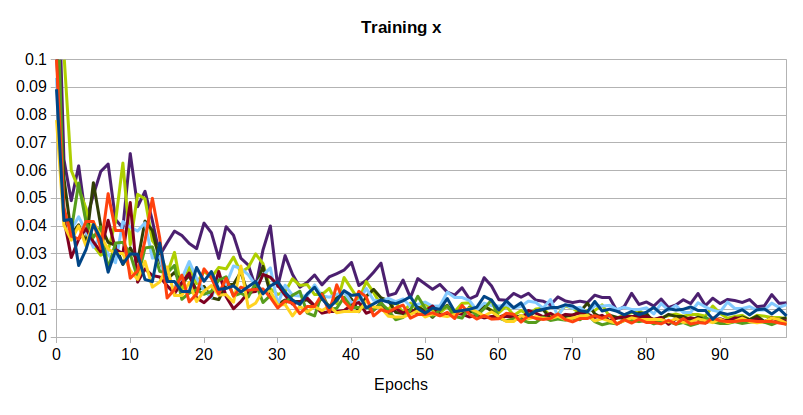
\includegraphics[width=0.45\textwidth]{Sistema de vision artificial/REGRESSION/train_x.png} &
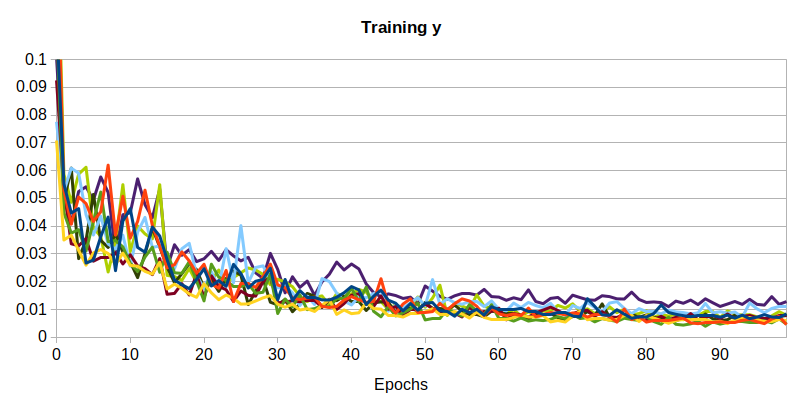
\includegraphics[width=0.45\textwidth]{Sistema de vision artificial/REGRESSION/train_y.png}
\end{tabular}
\begin{tabular}{c}
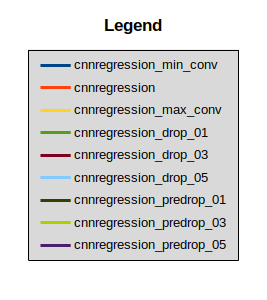
\includegraphics[width=0.3\textwidth]{Sistema de vision artificial/REGRESSION/legend.png}
\end{tabular}
\caption{Comparativa de las fases de entrenamiento del regresor}
\label{chap:Generación de un dataset fig:Entrenamiento Regresor}
\end{figure}

\begin{figure}[ht]
\centering
\begin{tabular}{cc}
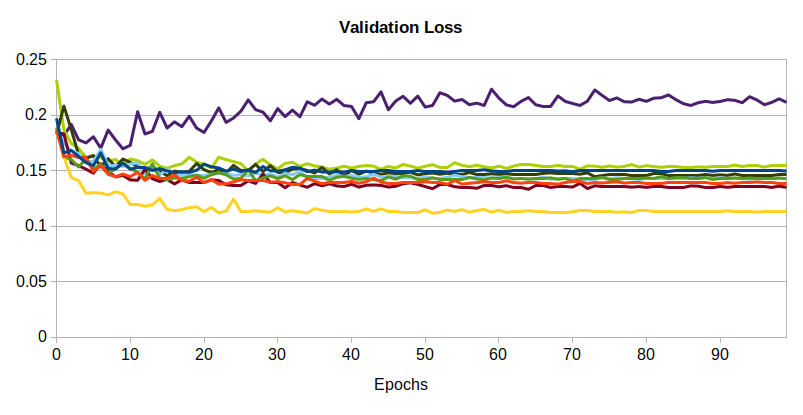
\includegraphics[width=0.45\textwidth]{Sistema de vision artificial/REGRESSION/val_loss.png} &
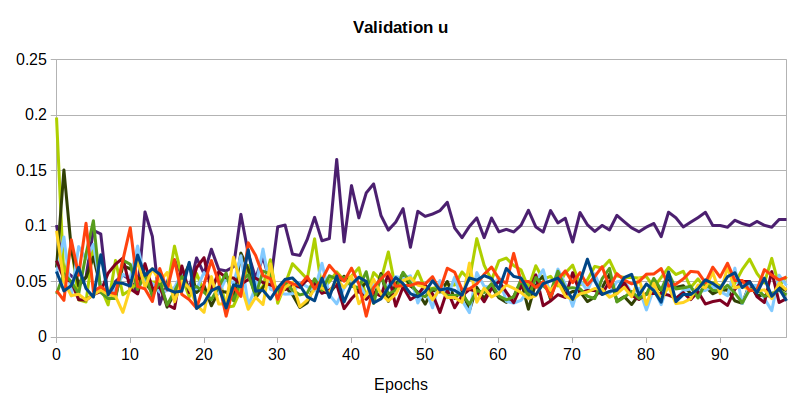
\includegraphics[width=0.45\textwidth]{Sistema de vision artificial/REGRESSION/val_u.png}
\end{tabular}
\begin{tabular}{cc}
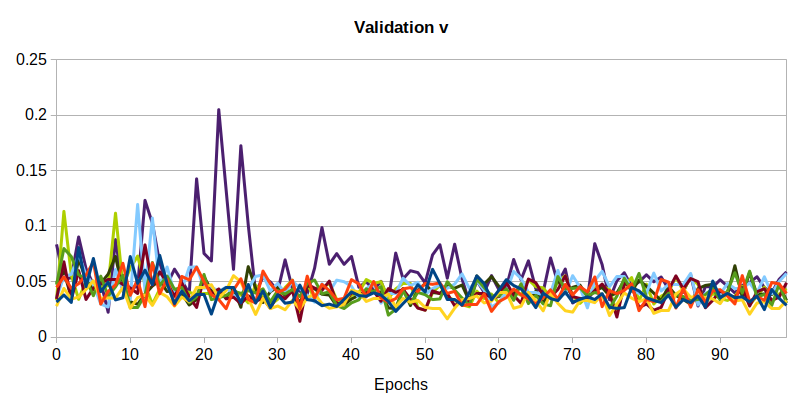
\includegraphics[width=0.45\textwidth]{Sistema de vision artificial/REGRESSION/val_v.png} &
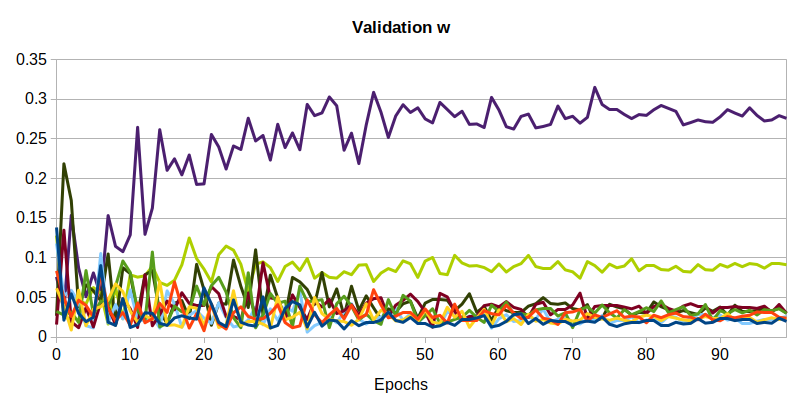
\includegraphics[width=0.45\textwidth]{Sistema de vision artificial/REGRESSION/val_w.png}
\end{tabular}
\begin{tabular}{cc}
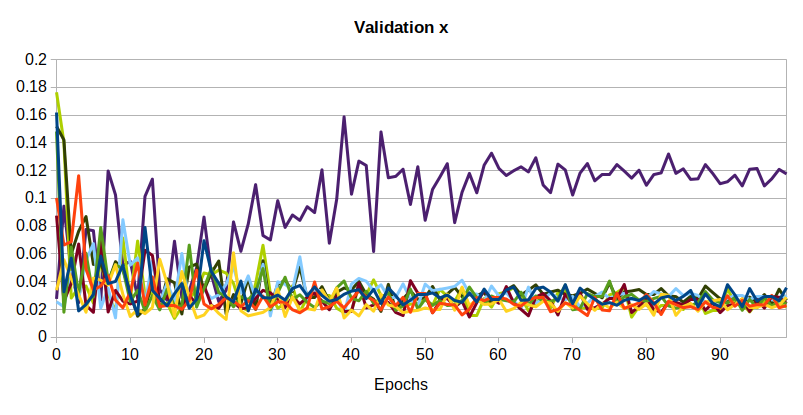
\includegraphics[width=0.45\textwidth]{Sistema de vision artificial/REGRESSION/val_x.png} &
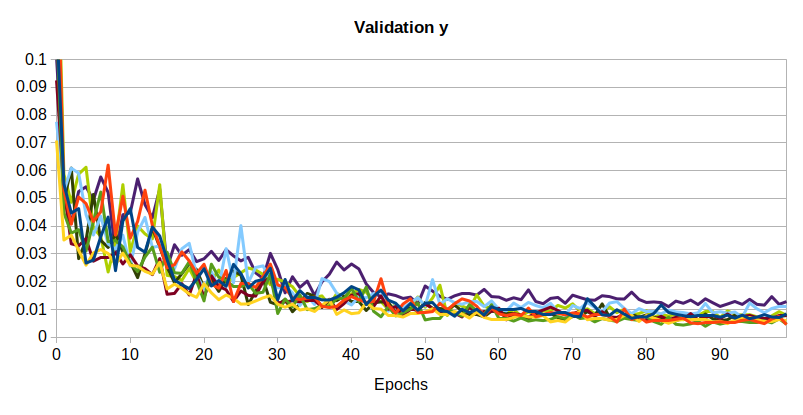
\includegraphics[width=0.45\textwidth]{Sistema de vision artificial/REGRESSION/val_y.png}
\end{tabular}
\begin{tabular}{c}
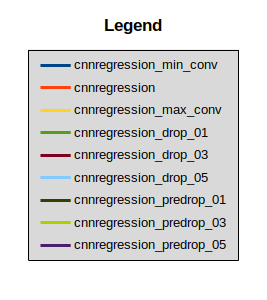
\includegraphics[width=0.3\textwidth]{Sistema de vision artificial/REGRESSION/legend.png}
\end{tabular}
\caption{Comparativa de las fases de validación del regresor}
\label{chap:Generación de un dataset fig:Validación Regresor}
\end{figure}